\documentclass[12pt,a4paper]{report}
\linespread{1.2}

\usepackage{amsmath,amssymb,amsfonts}
\usepackage{algorithmic}
\usepackage{graphicx}
\usepackage{xcolor}
\usepackage{multirow}
\usepackage{float}
\usepackage{listings}
\usepackage{listings-golang}
\lstset{ % add your own preferences
    frame=single,
    basicstyle=\linespread{0.9}\footnotesize\ttfamily,
    keywordstyle=\color{red},
    numbers=left,
    numbersep=5pt,
    showstringspaces=false, 
    stringstyle=\color{blue},
    tabsize=4,
    language=Golang % this is it !
}
% \lstdefinelanguage{yaml}{
%   keywords={true,false,null,y,n},
%   keywordstyle=\color{darkgray}\bfseries,
%   ndkeywords={},
%   ndkeywordstyle=\color{black}\bfseries,
%   identifierstyle=\color{black},
%   sensitive=false,
%   %moredelim=[l]{}{:},
%   comment=[l]{#},
%   morecomment=[s]{/*}{*/},
%   commentstyle=\color{purple}\ttfamily,
%   stringstyle=\color{blue}\ttfamily,
%   %morestring=[l]{-}{},
%   morestring=[b]',
%   morestring=[b]"
% }
\usepackage[font={small,it}]{caption}
\usepackage[english,ngerman]{babel}
\usepackage[backend=biber,
            sorting=none,   % Keine Sortierung
            doi=true,       % DOI anzeigen
            isbn=true,      % ISBN nicht anzeigen
            url=true,       % URLs anzeigen
            maxnames=6,     % Ab 6 Autoren et al. verwenden
            minnames=1,     % und nur den ersten Autor angeben
            style=numeric-comp,]{biblatex}
\addbibresource{literatur.bib}
\usepackage[colorlinks=true,
            urlcolor=black,
            linkcolor=black,
            filecolor=black,
            citecolor=black,]{hyperref}
\usepackage{fancyhdr}
% \pagestyle{fancy}
% \fancyhf{}
% \rhead{\thechapter}
% \cfoot{\thepage}

\def\BibTeX{{\rm B\kern-.05em{\sc i\kern-.025em b}\kern-.08em
    T\kern-.1667em\lower.7ex\hbox{E}\kern-.125emX}}

\begin{document}

\title{Erzeugung, Aufzeichnung und Wiedergabe von Netzwerk-Unterbrechungen in einer Testumgebung für verteilte Systeme}


\author{Jonathan Arns
	\textit{Hochschule Mannheim} \\
	Fakultät für Informatik\\
	Paul-Wittsack-Str. 10\\
	68163 Mannheim\\
	jonathan.arns@stud.hs-mannheim.de
}

\maketitle

\tableofcontents
% \setlength{\parindent}{0em}
\setlength{\parskip}{0.6em}

%%%%%%%%%%%%%%%%%%%%%%%%%%%%%%%%% Document beginning %%%%%%%%%%%%%%%%%%%%%%%%%%%%%%%%%%%%%%

\begin{abstract}
	Das ist das abstract, das werde ich wohl am Ende schreiben.
\end{abstract}


\chapter{Einleitung}
\cite{analysis_of_network_partition_failures}
\chapter{Grundlagen}
\section{Verteilte Systeme}
\subsection{Partition Tolerance}
\subsection{CAP}
\subsection{Linearisierbarkeit}
\subsection{Verteilter Consens}
\section{Docker}
Docker als leichtgewichtige Alternative zu virtuellen Maschinen ist inzwischen weitgehen bekannt und bildet das Rückrad vieler
moderner Cloud Anwendungen. Verteilte Microservice-basierte Systeme laufen heute fast ausschließlich in Containern und damit oft
in Docker oder ähnlichen Technologien.
\section{Proxy}

\chapter{Stand der Technik}
Im Umgang mit Fehlern in verteilten Systemen werden eine Reihe verschiedener Ansätze mit unterschiedlichen Zielen verfolgt.
Failure Testing und Chaos Engineering sind zwei ähnliche Methoden, die sich darauf verlassen, Fehler mit Hilfe von Tests zu
finden, mit dem Unterschied, dass Failure Testing in einer Test-Umgebung und Chaos Engineering in der Produktions-Umgebung
stattfinden. Daneben gibt es Log-Analyse und Tracing Systeme, die vor allem dazu dienen, aufgetretene Fehler nachzuvollziehen. Zu
diesem Zweck gibt es ebenfalls eine Handvoll weiterer, oft experimenteller Debugging Tools. Diese reichen von Tools, die einem
normalen Debugger ähneln, bis hin zu Tools, die sich vor allem auf die Visualisierung von Systemen und Abläufen konzentrieren.
Nachfolgend werden die genannten Methoden und jeweils wichtige Tools weiter erläutert.
\cite{challenges_and_options}

\section{Failure Testing}
Failure Testing ist ein Ansatz zum Testen der Fehlertoleranz verteilter Systeme. Die Grundidee ist immer, als Client mit dem
System zu interagieren und zeitgleich die Umgebung des Systems zu manipulieren, beispielsweise mit Netzwerk-Unterbrechungen.
Failure Tests werden als automatisierte Integrationstests über eine Programmierschnittstelle definiert und umfassen in der Regel den Aufbau
und Abbau des Systems, eine Reihe definierter Interaktionen mit dem System und zufällige oder deterministische Fehler-Injektionen
in die Systemumgebung. Zusätzlich wird oft nach Tests die Einhaltung von Invarianten des Systems anhand eines Modells geprüft, um
in zufallsgetriebenen Tests automatisch Bugs identifizieren zu können. \cite{failify_masters_thesis}

Majumdar et. al. \cite{why_is_random_testing_effective} zeigen, dass zufallsgetriebenes Failure-Testing effektiv für
Partition-Toleranz Bugs ist, obwohl die Menge an potentiell fehlerhaften Abläufen in realen Systemen gewaltig ist. Diese
Effektivität zeigt sich auch in der Realität an Tools wie Jepsen. Jepsen ist ein Failure-Testing-Framework in der Sprache
Clojure, welches speziell auf das Verhalten von verteilten Systemen bei Netwerk-Unterbrechungen u.Ä. ausgerichtet ist. Jepsen hat
sich auf dem Gebiet zu einem Industriestandart für das Testen von verteilte Datenbanken entwickelt \cite{abstracting_the_geniuses}
und wird für Projekte wie MongoDB, etcd, VoltDB, Hazelcast, Elasticsearch und CockroachDB verwendet und hat in jedem dieser
Systeme bereits reale Bugs aufgedeckt \cite{jepsen_analyses}.

Bei Jepsen-Tests werden auf einem Kontrollknoten eine Reihe von Client Prozessen ausgeführt, die Requests an das SUT senden.
Gleichzeitig werden mit Hilfe von sog. Nemesis Prozessen zufallsbasiert verschiedene Fehler in das System eingeführt. Zur
Erzeugung von Netzwerk-Unterbrechungen verwendet Jepsen die in Linux integrierten Netwerk-Tools auf den jeweiligen Knoten des SUT.
Neben Netzwerk-Unterbrechungen ist Jepsen in der Lage, verschiedene andere Fehler zu erzeugen, wie beispielsweise Unterschiede
zwischen den Systemuhren der einzelnen Knoten.  Am Ende eines Tests wird verifiziert, ob alle durchgeführten Operationen unter den
Regeln des SUT linearisierbar sind. Sind sie das nicht, hat Jepsen einen Bug gefunden. \cite{jepsen_github}

Failure-Testing eignet sich vor allem gut für Komponenten mit hohen Anforderungen an Fehlertoleranz und Korrektheit, wie verteilte
Datenbanken, Message-Broker und verteilte Dateisysteme. Failure-Testing ist heute der effektivste Ansatz, um Bugs in solchen
Systemen zu finden \cite{abstracting_the_geniuses} und der hohe Aufwand Failure-Tests einzurichten, lohnt sich hier besonders, da
diese Systeme in der Regel eine große Menge von Nutzern haben, die sich auf deren Zuverlässigkeit verlassen.

\section{Chaos Engineering}
Chaos Engineering verfolgt das Ziel, die Resilienz und Verfügbarkeit von großen, heterogenen verteilten Systemen in Produktion zu
verbessern. Dazu werden direkt in der Produktions-Umgebung Experimente mit Fehlern wie Abstürzen von Virtuellen Maschinen und
Netwerk-Unterbrechungen durchgeführt, um Schwachstellen zu identifizieren und zu verifizieren, dass das System im Ernstfall mit
derartigen Fehlern umgehen kann. Basiri et. al. \cite{chaos_engineering}, die Chaos Engineering, wie es bei Netflix eingesetzt
wird, vorstellen, definieren den Ablauf eines Experiments dabei in vier Schritten.
\begin{enumerate}
	\item Definiere den Ruhezustand des Systems anhand vorhandener Ausgaben Systems.
	\item Erwarte, dass der Ruhezustand sowohl in der Kontrollgruppe, als auch in der Versuchsgruppe bestehen bleibt.
	\item Injiziere Ereignisse wie Server-Abstürze und Netzwerk-Unterbrechungen in der Versuchsgruppe von Services.
	\item Versuche die Hypothese anhand der Unterschiede zwischen Kontroll- und Versuchsgruppe zu widerlegen.
\end{enumerate}
Bekannt gemacht wurde die Methode durch Netflix \cite{abstracting_the_geniuses}, unter anderem mit dem dort entwickelten Chaos
Monkey. Dieser ist ein Service, der automatisiert während der normalen Arbeiteszeiten Fehler im Produktionssystem erzeugt. Die
injizierten Fehlern sind dabei Abstürze von internen Services, Abstürze von virtuellen Maschinen und Netzwerk-Unterbrechungen und
Netzwerk-Latenz für einzelne Nachrichten. Netflix stellt heraus, dass als Folge dessen Entwickler ihre Services resilient gegen
dearartige Fehler bauen und die Verfügbarkeit des Systems sich dadurch deutlich verbessert. Zusätzlich zu automatisierten Tools
wie dem Chaos Monkey wird beim Chaos Engineering auf manuelle Experimente gesetzt, die Teilweise sehr große Störungen wie
Netzwerk-Unterbrechungen zu großen Teilen des Systems in Form von ganzen AWS Regionen umfassen. Erweisen sich manuelle Experimente
als effektiv, werden diese wiederum nach und nach automatisiert. \cite{chaos_engineering}

Chaos Engineering eignet sich besonders gut für sehr große, heterogene Systeme bei großen Organisationen wie Netflix, die in der
Lage sind, spezialisierte Chaos Engineers einzustellen oder auszubilden. Dort hat sich die Methode aus der Not heraus als Best
Practice und fester Teil der Engineering Kultur etabliert. \cite{abstracting_the_geniuses}

\section{Log-Analyse}
Log Analyse ist ein leichtgewichtiger Black-Box Ansatz zur Fehleridentifikation und -Analyse, der sich für Systeme eignet, welche
nicht modifiziert werden können \cite{challenges_and_options}. Es werden so viele Logs wie möglich aus den
verschiedenen Teilen eines Systems aggregiert und gemeinsam analysiert. Aufgrund der großen Menge an Logs sind diese allein oft
nicht direkt für einen Menschen verwendbar. Stattdessen werden Data-Mining-Techniken eingesetzt, um nützliche Information aus den
aggregierten Logs zu extrahieren \cite{log_analysis_at_google}.

\section{Tracing}
Eine deutlich schwergewichtigere Lösung ist das Tracing eines verteilten Systems. Die Idee ist, jede Aktion, die im Zusammenhang
mit einem User-Request passiert, aggregiert aufzuzeichnen, um so den gesamten Weg eines Requests durch das System zeigen zu können.
Dabei können verschiedene Informationen aufgezeichnet werden, unter anderem Log Nachrichten und RPC Aufrufe, bzw. interne
Nachrichten, je nach dem, was das Ziel des konkreten Tracing Systems ist. Im Gegensatz zur einfachen Log Analyse erfordert Tracing
Eingriffe in das verteilte System, um die notwendigen Informationen zu generieren und mit Trace-IDs zu kennzeichnen. Die erzeugten
Traces können dafür in der Regel gut visualisiert werden und bieten Entwicklern in dieser Form direkt nützliche Einsichten in das
System. \cite{dapper_tracing}

Tracing ist eine vielseitige Methode, die je nach Implementierung unterschiedliche Use-Cases bedienen kann. Neben verteiltem
Profiling zur Identifikation von Bottlenecks im System und der Diagnose von Problemen im Ruhezustand des Systems zählt
Anomalieerkennung in verteilten Systemen zu diesen Use-Cases. Dazu gehört sowohl die Erkennung, als auch das Debugging von selten
auftretenden Problemen, die beispielsweise durch Netzwerk-Unterbrechungen ausgelöst werden können. \cite{so_you_want_to_trace}

Ähnlich wie Chaos Engineering wird Tracing von Organisationen mit großen, heterogenen Systemen in Produktions-Umgebungen
eingesetzt. Mit Dapper \cite{dapper_tracing} hat Google eine eigene Tracing Lösung geschaffen, die sich vor allem für das
Profiling von Systemen und die Diagnose von Problemen im Ruhezustand des Systems eignet \cite{so_you_want_to_trace}. Magpie
\cite{magpie_tracing} ist ein Tracing System, welches sich insbesondere zur Annomalieerkennung eignet, sowohl für Probleme in der
Korrektheit, als auch der Performance von verteilten Systemen \cite{so_you_want_to_trace}.

\section{Debugging}
Neben Werkzeugen wie Tracing, die ebenfalls zum Debugging von verteilten Systemen dienen gibt es eine Reihe weiterer Tools, die
konkret diesem Zweck dienen, oft mit einem speziellen Fokus auf entweder eine bestimmte Art von Systemen oder eine bestimmte
Klasse von Fehlern. Die Tools lassen sich in zwei grobe Kategorien einteilen: Visuelle Debugger und Klassische Debugger.

\subsection{Interaktives Debugging}
Die Tools in dieser Kategorie versuchen, die interaktive Debugging-Erfahrung von nicht-verteilten Systemen mit Debuggern wie GDB auf verteilte
Systeme zu übertragen. Die Herausforderung dabei ist, dass klassische Debugger darauf ausgelegt sind, genau einen Prozess
zu kontrollieren, in verteilten Systemen aber per Definition mehrere Prozesse, oft auf verschiedenen Rechnern, existieren.
Zusätzlich zu Kontrollfluss und Zustandsänderungen in einzelnen Prozessen müssen durch die Verteiltheit des Systems ebenfalls
Nachrichtenflüsse zwischen den Prozessen beobachtet werden. Achar et. al. \cite{gotcha_interactive_debugger} stellen heraus, dass
interaktives Debugging im klassischen Sinne in verteilten Systemen nicht im generellen Fall möglich ist. Stattdessen muss ein
System gewisse Einschränkungen im Bezug auf Zustandsänderungen und die Trennung zwischen lokalen und geteilten Zuständen
einhalten. Mit GoTcha \cite{gotcha_interactive_debugger} stellen sie einen vollständigen interaktiven Debugger für Systeme mit dem
Global Object Tracker (GoT) Programmiermodell vor. Konkret funktioniert GoTcha nur für Systeme, die eine GoT Implementierung in
Python namens Spacetime verwenden. Damit ist GoTcha zwar für solche Systeme ein mächtiges Tool, in seiner Anwendbarkeit aber enorm
eingeschränkt.

Ein anderer Ansatz, der eine interaktive Debugging-Erfahrung erzielen kann, der auch in nicht-verteilten Systemen Anwendung findet
\cite{normal_record_and_replay}, um besonders flüchtige Bugs zu reproduzieren, ist Record-and-Replay Debugging. Dieser Ansatz
wurde erstmals bereits 1997 auch auf verteilte Systeme angewandt \cite{distributed_replay_debugging_1997}, damals im Modul für
verteilte Applikationen des Compilers der Programmiersprache Ada95. Damit konnten Abläufe von verteilten Systemen aufgezeichnet
werden, um dann zu Debugging Zwecken die Abläufe auf einzelne Knoten des Systems wiederzugeben.

Ein etwas moderneres Beispiel für die gleiche Idee ist liblog \cite{distributed_replay_debugging_2006}, ein Record-and-Replay Debugger für
C und C++ Applicationen, der in der Lage ist, Netzwerk Verkehr mit aufzuzeichnen. Der Mechanismus hinter liblog ist, alle
Systemaufrufe, die eine Applikation macht, zu loggen, so dass diese später deterministisch wiedergegeben werden können.

\subsection{Visuelles Debugging}
Ein Problem des klassischen interaktiven Debugging Ansatzes ist, alle relevanten Informationen verständlich darzustellen. Das
liegt daran, dass nicht nur die Zustände der einzelnen Knoten, sondern als zusätzliche Ebene auch die Kommunikation
zwischen den Knoten relevant ist. Die Problematik wird unter anderem dadurch deutlich, dass liblog beispielsweise gleich mehrere
GBD Instanzen als Frontend für Replays benötigt \cite{distributed_replay_debugging_2006}.

Um das Problem zu lösen haben sich mit der Zeit eine Reihe von Debugging Tools für verteilte Systeme entwickelt, die sich darauf
konzentrieren, Abläufe und Zustände auf Systemebene zu visualisieren. Ein gemeinsames Konzept der verschiedenen Lösungen ist die
Verwendung von Zeit-Raum-Diagrammen zur visualisierung von Events und Nachrichtenflüssen zwischen den einzelnen Knoten. Ein
Beispiel hierfür ist in Abbildung \ref{fig:shiviz} dargestellt, diese zeigt ein interaktives Zeit-Raum-Diagramm aus dem Tool
ShiViz \cite{ShiViz_visual_debugger}, welches zusätzliche Detailinformationen zu Events anbietet.

\begin{figure}[H]
	\centering
	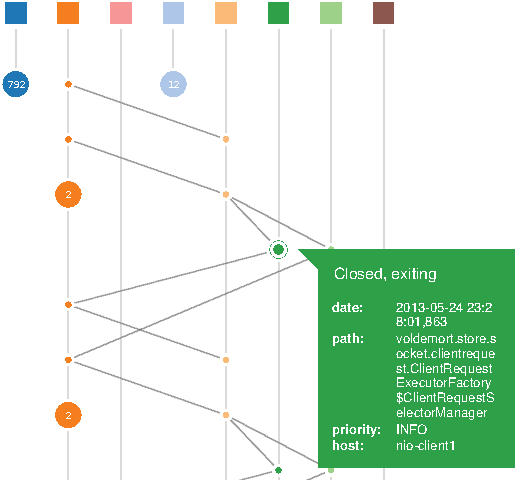
\includegraphics[width=\linewidth]{img/shiviz_time_space.pdf}
	\caption{Interaktives Raum-Zeit-Diagramm in Shiviz \cite{ShiViz_visual_debugger}}
	\label{fig:shiviz}
\end{figure}

Ein sehr mächtiger visueller Debugger ist Oddity \cite{oddity_graphical_debugger}. Das Tool bietet eine interaktive Debugging
Erfahrung, die in vielen Aspekten normalen Debuggern ähnelt, allerdings nur auf Systemebene. Oddity erlaubt es, die Ausführung von
einzelnen Knoten des SUT zu pausieren, sowie einzelne Nachrichten und Events zu kontrollieren, alles in einer graphischen
Oberfläche, die den Zustand des Systems inklusive Events und Nachrichten darstellt. Ein Screenshot dieser Darstellung ist in
Abbildung \ref{fig:oddity} zu sehen. Oddity erlaubt es außerdem den Systemzustand zu einem früheren Zustand zurück zu setzen und
so mehrere Kontrollflüsse in einer Session zu debuggen. Zusätzlich zu der graphischen Oberfläche, die live den Systemzustand
abbildet, kann Oddity auch Zeit-Raum-Diagramme für Abläufe des Systems generieren.

Bei all diesen Vorzügen hat Oddity zwei große Einschränkungen. Einerseits funktioniert das Tool aktuell nur für Systeme, die als
eine Sammlung von Event Handlern implementiert sind. Andererseits erfordert Oddity erheblichen Aufwand zur Einrichtung, da eine
auf das konkrete SUT zugeschnittene Implementierung einer Oddity API erforderlich ist, die direkt mit dem SUT interagieren kann.
Die erste Einschränkung ist nicht inherent und Woos et. al. \cite{oddity_graphical_debugger} schreiben, dass in Zukunft ohne Probleme weitere
Programmiermodelle unterstützt werden können. Der Einrichtungsaufwand dagegen ist tiefer in der Architektur des Tools verankert und
ist zur Umsetzung der vollen Funktionalität notwendig.

\begin{figure}[H]
	\centering
	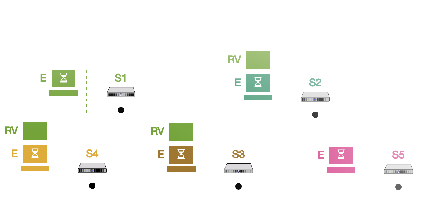
\includegraphics[width=\linewidth]{img/oddity_raft_state.pdf}
	\caption{Visualisierung eines Systemzustands in Oddity \cite{oddity_graphical_debugger}}
	\label{fig:oddity}
\end{figure}

Neben Tools wie ShiViz und Oddity, welche mindestens in ihren jeweiligen akademischen Umfeldern erfolgreich eingesetzt werden
\cite{ShiViz_usage_study, oddity_usage_in_education}, gibt es im Bereich der Visualisierung von verteilten Systemen auch Forschung
zum Einsatz von Augmented Reality. Mit debugAR stellen Reipschläger et. al. \cite{debugAR_AR_debugger} einen Prototypen vor, der
demonstriert, wie Augmented Reality verwendet werden könnte, um die vielen Dimensionen verteilter Systeme zu visualisieren.
Abbildung \ref{fig:debugAR} zeigt ein Rendering von debugAR, dargestellt ist ein interaktives Zeit-Raum-Diagramm ähnlich der
Oberfläche von ShiViz.

\begin{figure}[H]
	\centering
	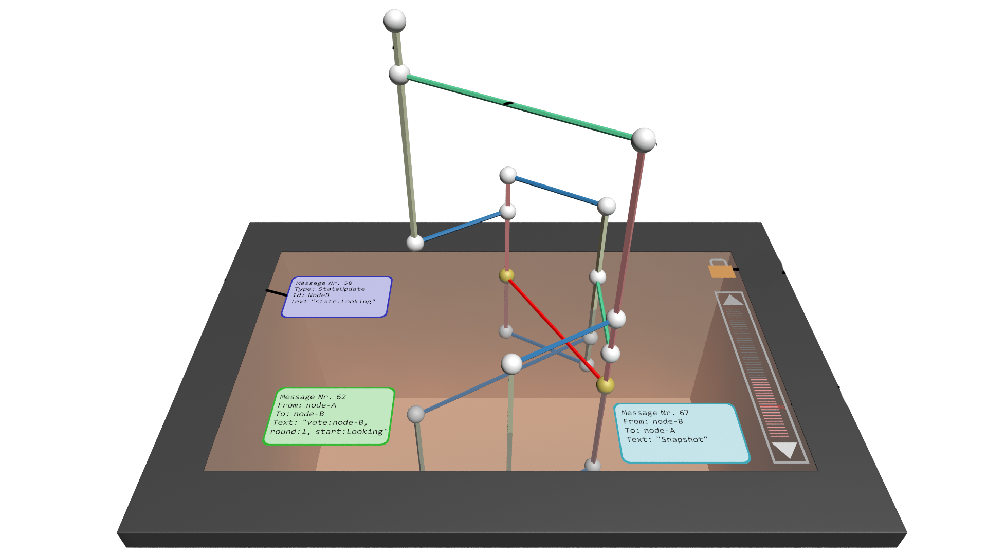
\includegraphics[width=\linewidth]{img/debugAR_rendering.png}
	\caption{Rendering einer 3D Visualisierung von Nachrichtenflüssen in debugAR \cite{debugAR_AR_debugger}}
	\label{fig:debugAR}
\end{figure}

\section{Was fehlt noch?}
Fehlertoleranz und Debugging in verteilten Systemen sind aktuelle Forschungsfelder, die sich schnell weiterentwickeln und
dementsprechend noch viele Möglichkeiten für Innovationen bieten. Die folgenden sind derzeit offene Probleme, die weiteren
Entwicklungen bedürfen.

\subsection{Failure-Testing und Chaos-Engineering}
Alvaro und Tymon \cite{abstracting_the_geniuses} stellen als großen aktuellen Mangel heraus, dass sowohl Failure-Testing, als auch
Chaos Engineering in der Anwendung so komplex sind, dass die Techniken ausschließlich den Entwicklern zur Verfügung stehen, die
sich voll darauf spezialisieren. Sie schlagen unter Anderem eine weitgehende Automatisierung von Failure-Testing in der Zukunft
vor. Ein weiteres Feld in dem Sie großes Potential zur Verbesserung sehen, sind Systeme, die die Erklärbarkeit von verteilten
Systemen verbessern und somit Entwicklern helfen, mittels Failure-Testing o. Ä. entdeckte Bugs besser nachvollziehen zu können.

Außerdem Fehlt der Industrie ein Failure-Testing Framework, welches es ermöglicht, effektiv Bugs aufzudecken diese Bugs mit
deterministischen Testfällen zu reproduzieren. Jepsen beispielsweise agiert ausschließlich zufallsbasiert und kann Bugs oft nicht
zuverlässig reproduzieren. Es ist außerdem wichtig, dass ein solches Framework cross-Plattform und Programmiersprachen-agnostisch
ist, um weitreichend einsetzbar zu sein. Heute verwenden einige große Projekte sogar noch eigens entwickelte Testing-Frameworks,
die sich auf ein konkretes System beschränken und durch den getrennten Entwicklungsaufwand nicht mit dem Funktionsumfang von Tools
wie Jepsen mithalten können. \cite{failify_masters_thesis}

Ebenfalls im Bezug auf allemeineres Tooling stellen Basiri et. al. \cite{chaos_engineering} die Fragen, ob sich allgemeineres
Tooling für Chaos-Engineering entwickeln lässt, da auch hier Organisationen ursprünglich vorwiegend eigene, interne Tools
entwickelt haben.

\subsection{Debugging}
Im Bereich des Debuggings von verteilten Systemen stellen sich ebenfalls noch eine Reihe von Herausforderungen für die Zukunft.
Unter Anderem die Frage danach, wie unterschiedliche Aspekte von verteilten Systemen am besten visualisiert werden können
\cite{oddity_graphical_debugger}. Auch ist noch offen, wie interaktive Debugger mit sehr großen Systemen skalieren können, sowohl
im Sinne der Visualisierung, als auch der Performance \cite{gotcha_interactive_debugger}.

Im Bereich der Replay-Debugger stellen Liu et. al. \cite{d3s_predicate_checker} im Kontext Ihres Prädikat-Checkers D3S
insbesondere offline-Replay als Teil Ihrer Zukunftsvision heraus, um mit D3S identifizierte Bugs einfach zu debuggen. In der
Praxis haben sich seitdem Failure-Testing und Chaos-Engineering gegenüber Prädikat-Checkern zur Bug-Identifikation durchgesetzt.
Nichts desto trotz könnte sich ein Programmiersprachen-agnostischer Replay-Debugger, welcher durch Failure-Testing gefundene Bugs
deterministisch wiedergeben kann, als sehr hilfreich erweisen und ist eine Entwicklung, die es noch zu machen gilt.



\chapter{Systembeschreibung}
Dieses Kapitel beschreibt die Idee, die Anforderungen und die Umsetzung des im Rahmen dieser Arbeit entwickelten Systems ditm.
\section{Idee}
Die grundlegende Idee dieser Arbeit ist ein Tool, welches die Ideen des Failure Testings mit denen des Record and Replay
Debuggings vereint. Dieses Tool soll nach Record and Replay Prinzip beim Debugging von Bugs im Zusammenhang mit
Netwerk-Unterbrechungen in verteilten Systemen helfen. Mit Hilfe des Tools sollen wie beim Failure Testing Netwerk-Unterbrechungen
während Test Durchläufen simuliert werden, allerdings nicht wie beim Failure-Testing in programmatisch von vorn herein definierten
Testfällen, sondern interaktiv, während der Nutzer mit dem System interagiert. Um gefundene Bugs dennoch zuverlässig reproduzieren
zu können, soll das Tool Situationen aufzeichnen und zum späteren Zeitpunkt wieder abspielen können, insbesondere mit den gleichen
simulierten Netzwerk-Bedingungen wie während der Aufzeichnung.

Ein großer Fokus der Arbeit ist dabei speziell auf dem verfolgten Ansatz für ein solches System. Dieser ist, alle Nachrichten
innerhalb eines verteilten Systems über einen Proxy zu leiten, der diese inklusive Metadaten aufzeichnet und in der Lage ist,
kontrolliert Netwerk-Unterbrechungen zu simulieren, indem einzelne Nachrichten geblockt, bzw. nicht weiter geleitet, werden.  Mit
diesem Aufbau soll auch ein Replay der Netzwerk-Bedingungen anhand eines zuvor durch den Proxy aufgezeichneten Test Durchlaufs
möglich sein, sofern der Proxy in der Lage ist, während des Replays für jeden erhaltenen Request zu identifizieren, welchem
Request aus der Aufzeichnung er jeweils zuzuordnen ist. Zudem muss der Proxy Requests, die in der Aufzeichnung von außerhalb des
Systems kamen, identifizieren und während des Replays zum richtigen Zeitpunkt selbstständig in das System senden.

Ein Proxy wird den anderen, verbreiteteren Fehler-Mechanismen des Failure-Testings vorgezogen, da die Erwartung ist, dass dieser
sich insbesondere besser für Replays eignet. Das liegt daran, dass ein Proxy jede Nachricht des SUT einzeln betrachten und
gegebenenfalls blocken kann, andere Mechanismen, die sich rein auf zeitliche Abstände und die Reihenfolge von Operationen
verlassen, ermöglichen dies nicht ohne weiteres. Dadurch soll das Tool besser mit Unterschieden in der zeitlichen Reihenfolge von
Nachrichten umgehen können, die im Replay auftreten können, zum Beispiel weil Replays schneller als das originale Recording
ablaufen, falls im Recording ein Mensch mit dem SUT interagiert hat, dessen Aktionen deutlich schneller als in Echtzeit agbespielt
werden.

\section{Anforderungen}
ditm ist ein Prototyp, der primär dem Zweck dient, die zuvor beschriebene Idee zu verfizieren.
Die Anforderung reflektieren diesem Umstand, indem beispielsweise die unterstützten Netwerk-Protokolle auf HTTP beschränkt sind.
\subsection{Funktionale Anforderungen}
\begin{table}[H]
	\centering
	\caption{Funktionale Anforderungen}
	\label{tab:fa}
	\begin{tabular}{|l|l|p{7cm}|}
		\hline
		ID   & Anforderung                   & Beschreibung                                                                                                                                                                                                          \\ \hline
		FA1  & Netzwerk Unterbrechungen      & Das System soll kontrolliert Netzwerk-Unterbrechungen zwischen Knoten des zu testenden Systems erzeugen können.                                                                                                       \\ \hline
		FA2  & Aufzeichnung                  & Das System soll den gesamten Netzwerkverkehr des zu testenden Systems aufzeichnen können. Insbesondere sollen auch erzeugte Netzwerk-Unterbrechungen aufgezeichnet werden.                                            \\ \hline
		FA3  & Replay                        & Das System soll anhand einer durch das System erstellten Aufzeichnung die Situation in der Aufzeichnung am laufenden Testsystem wiederherstellen und vor allem inklusive Netzwerk-Unterbrechungen wiedergeben können. \\ \hline
		FA4  & Zufällige Unterbrechungen     & Das System soll Netwerk-Unterbrechungen zufällig erzeugen können.                                                                                                                                                     \\ \hline
		FA5  & Kontrollierte Unterbrechungen & Das System soll dem Nutzer die Möglichkeit geben, Netwerk-Unterbrechungen konkret zu steuern.                                                                                                                         \\ \hline
		FA6  & Log Aggregation               & Das System soll zusätzlich zum Netzwerkverkehr auch die Log ausgaben des zu testenden Systems aufzeichnen und aggregieren können.                                                                                     \\ \hline
		FA7  & Log Matching                  & Das System soll die aufgezeichneten Nachrichten und Logs in chronologischer Reihenfolge gemeinsam anzeigen können.                                                                                                    \\ \hline
		FA8  & Volume Snapshots              & Das System soll für zustandsbehaftete Systeme Snapshots der Docker Volumes erstellen und zu einem späteren Zeitpunk wiederherstellen können.                                                                          \\ \hline
		FA9  & Nachrichten von außen         & Das System soll dem Nutzer Schnittstelle bieten, über die Nachrichten reproduzierbar von außen in das zu testende System gesendet werden können, um Prozesse im zu testenden System anzustoßen.                       \\ \hline
		FA10 & Responses Blocken             & Das System soll in der Lage sein, nicht nur Requests auf dem Hinweg zum Server zu blockieren, sondern optional auch erst die Antwort auf dem Rückweg.                                                                 \\ \hline
	\end{tabular}
\end{table}

\subsection{Nicht-Funktionale Anforderungen}
\begin{table}[H]
	\centering
	\caption{Nicht-Funktionale Anforderungen}
	\label{tab:nfa}
	\begin{tabular}{|l|l|p{7cm}|}
		\hline
		ID   & Anforderung              & Beschreibung                                                                                                                                                                                                  \\ \hline
		NFA1 & Portabilität             & Das System soll vollständig in Docker lauffähig sein und mittlels docker-compose konfigurierbar sein.                                                                                                         \\ \hline
		NFA2 & Proxy Architektur        & Umsetzung des Konzepts, einen Proxy zur erzeugung etc von Partitionen zu verwenden                                                                                                                            \\ \hline
		NFA3 & HTTP                     & Das System soll mit HTTP als Netzwerkprotokoll Arbeiten und grundlegend alle verteilten Systeme, die ausschließlich über HTTP kommunizieren und die Umgebungsvariable HTTP\_PROXY respektieren, unterstützen. \\ \hline
		NFA4 & Deterministische Replays & In der Wiedergabe einer Aufzeichnung sollen immer genau die Teile des Netzwerkverkehrs geblockt werden, die auch in der Aufzeichnung vom System geblockt wurden. Nicht mehr, nicht weniger und keine anderen. \\ \hline
		NFA5 & Usability                & Das System soll einfach über eine graphische Oberfläche bedienbar sein.                                                                                                                                       \\ \hline
		NFA6 & Echtzeit                 & Requests und Logs einer laufenden Aufzeichnung sollen in Echtzeicht angezeigt werden.                                                                                                                         \\ \hline
		NFA7 & Default Test System      & Das zu testenden System sollte für den Test nicht angepasst werden müssen.                                                                                                                                    \\ \hline
	\end{tabular}
\end{table}

\section{Architektur}
Das Herzstück des Systems ist entsprechend der Idee ein eigens entwickelter HTTP Proxy, welcher den Netzwerk-Verkehr in einem
verteilten System aufzeichnen und Nachrichten wahlweise nicht weiter leiten kann. Dieser Proxy läuft in einem Docker Container
direkt neben dem SUT und ist auch Teil des gleichen Docker Netzwerks wie das SUT. Außer dem Proxy hat ditm eine weitere eigens
entwickelte Komponente, ein Docker-Log-Driver-Plugin, welches Container-Logs an den Proxy sendet. Die Datenflüsse zwischen
Komponenten des Systems sind in Abbildung \ref{fig:dataflow} im Kontext eines SUT mit zwei Knoten dargestellt.
\begin{figure}[H]
	\centering
	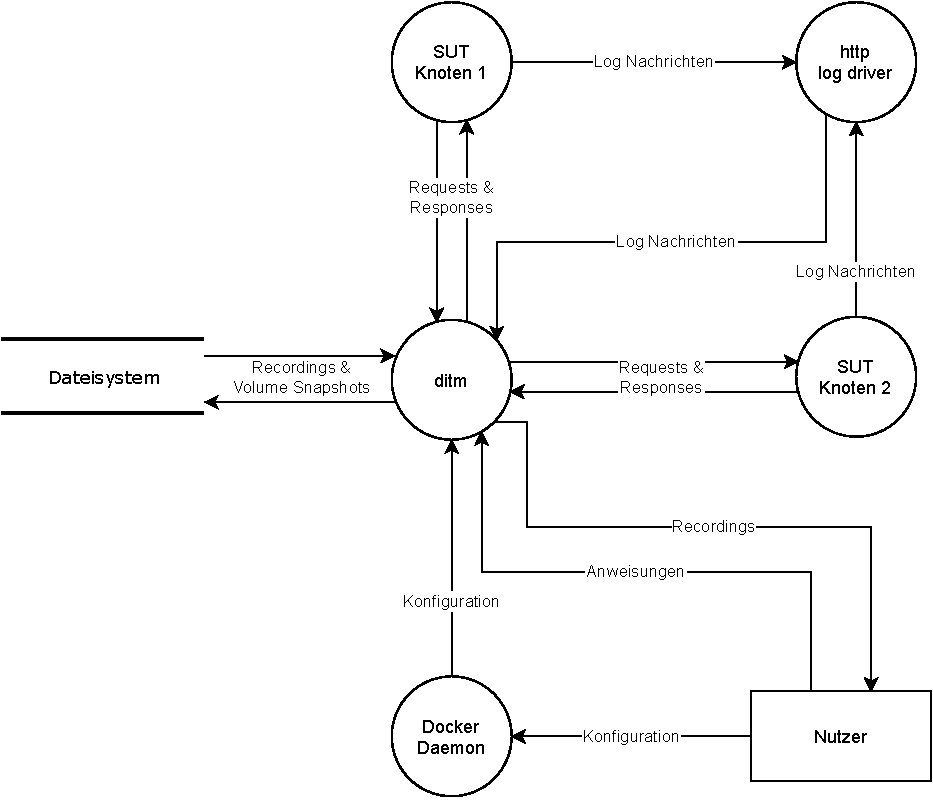
\includegraphics[width=\linewidth]{img/ditm-Dataflow.pdf}
	\caption{Datenflussdiagramm für ditm}
	\label{fig:dataflow}
\end{figure}

\subsection{Datenmodell}
Das Datenmodell von ditm ist einfach gehalten. Das Top Level Datenobjekt ist das Recording, dieses enthält zwei chronologisch
geordnete Listen, eine mit den Log Nachrichten des SUT und eine mit den aufgezeichneten Requests. Beide Listen enthalten
die jeweiligen Objekte für alle Knoten des SUT, ohne diese weiter voneinander zu trennen. Sollte eine gefilterte Liste
benötigt werden, die nur Objekte für bestimmte Knoten enthält, wird diese dynamisch erzeugt. Recordings enthalten außerdem
eine Referenz auf einen Volume Snapshot, sofern für das Recording einer existiert.
Die eigentlichen Request Datenobjekte enthalten neben dem Request Body eine Menge Metadaten, die teilweise vom Request selbst
stammen und teilweise durch ditm erzeugt wurden, beispielsweise ob der Request geblockt wurde oder nicht.
Log Nachrichten umfassen neben der eigentlichen Nachricht ebenfalls wichtige Metadaten, wie den Namen des Containers, der die
Nachricht geloggt hat. In Abbildung \ref{fig:class} ist das beschriebene Datenmodell in einem Klassendiagramm dargestellt. Die
Implementierungen des Matcher-Interfaces fehlen im Klassendiagramm, da sich hier keine Unterschiede zwischen den einzelnen
Implementierungen zeigen würden und diese gesondert in Kapitel ... behandelt werden. Die Methoden der Klasse Proxy wurden
ebenfalls aus Platzgründen weg gelassen und da diese hier konkret von geringerem Interesse sind. Ein Proxy nimmt im Prototypen die
Rolle eines Gottobjekts ein, dieses Design-Pattern wurde für den Prototypen solideren Patterns vorgezogen, um die Entwicklung
einfach zu halten und Erweiterungen, bzw. Änderungen des Datenmodells währenddessen zu erleichtern.
\begin{figure}[H]
	\centering
	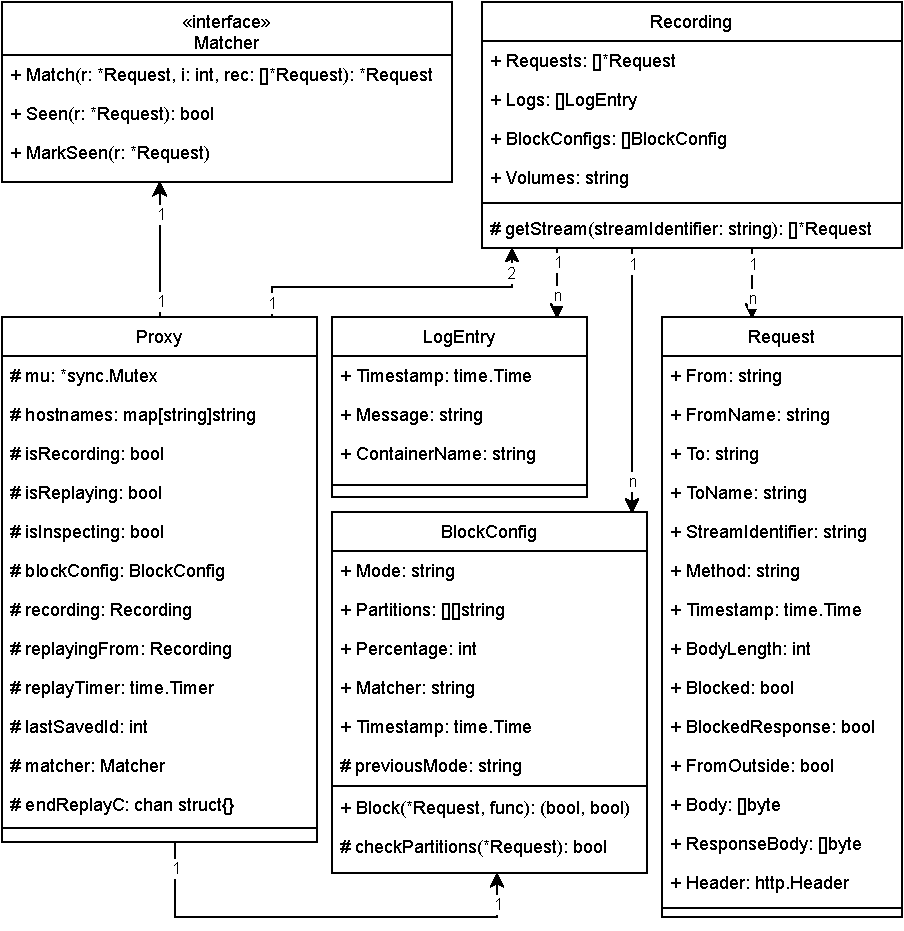
\includegraphics[width=\linewidth]{img/ditm-Class.pdf}
	\caption{Klassendiagramm für ditm ohne Proxy-Methoden und Matcher-Implementierungen}
	\label{fig:class}
\end{figure}

\subsection{Weg eines Requests}
Um eine konkrete Vorstellung von der Arbeitsweise des Proxys zu vermitteln, wird im folgenden beispielhaft der Weg eines
Requests durch das System beschrieben. In diesem Kontext wird der Ursprung des Requests als Client und das Ziel des
Requests als Server bezeichnet, beide sind Knoten des SUT. Abbildung \ref{fig:activity} stellt zunächst den groben Ablauf auf Systemebene dar.
Wichtig ist zu bemerken, dass der Proxy bereits beim ersten erhalten des Requests die komplette Analyse durchführt und
nicht nur entscheidet, ob der Request geblockt werden soll, sondern die Entscheidung auch direkt für die Response trifft,
ohne die Response jemals gesehen zu haben. Tatsächlich wird die Response gar nicht von ditm betrachtet, stattdessen wird
die Analyse vollständig am Request durchgeführt. Die einzige Interaktion des Proxys mit der Response ist, diese zur Anzeige im
Frontend aufzuzeichnen, sie zu blocken falls vorher festgelegt oder sie ansonsten direkt weiter zu leiten.
Der Grund dafür ist, dass fast alle für ditm relevanten Metadaten bereits aus dem Request abgeleitet werden können. Zwar
könnten die Länge der Response und die Response Header möglicherweise ebenfalls von Interesse sein, der Kompromiss wird
hier aber in Kauf genommen, da das die Implementierung erheblich vereinfacht und auch so genügend Metadaten vorliegen,
um verschiedene Algorithmen zur Entscheidung, ob ein Reqeust im Replay geblockt werden soll, zu evaluieren.
Die verschiedenen Ansätze, die diese Arbeit betrachtet, werden in Kapitel ... behandelt.
\begin{figure}[H]
	\centering
	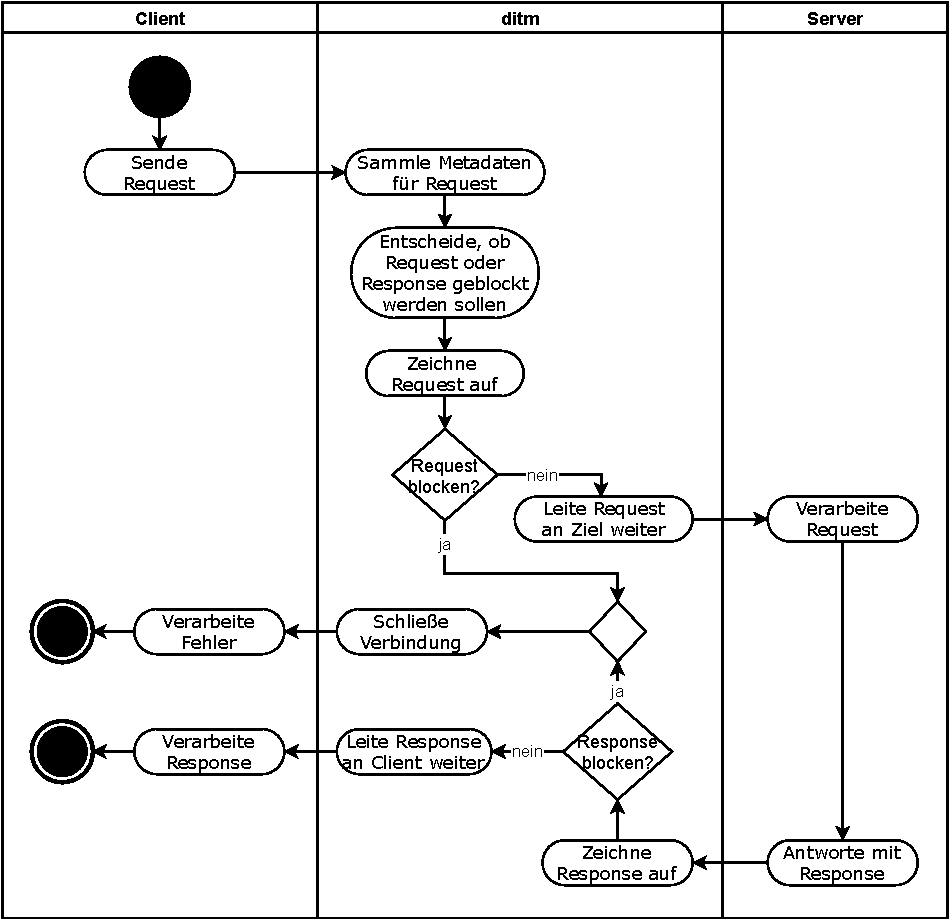
\includegraphics[width=\linewidth]{img/ditm-Activity.pdf}
	\caption{Aktivitätsdiagramm der Interaktion von ditm mit Client und Server eines Requests}
	\label{fig:activity}
\end{figure}

\section{Implementierung}
Als Programmiersprache wird für die Implementierung auf Go gesetzt. Go bietet sich an, da die Standartbibliothek
umfassende, robuste APIs für den Umgang mit Netzwerken bietet und die Sprache insgesamt eine schnelle
Entwicklungsgeschwindigkeit erlaubt, ohne Performance zu vernachlässigen.
\subsection{Datenspeicherung}
Als Speicherformat für ditm wurden einfache Dateien in JSON Format gewählt. So wird jedes Recording Datenobjekt in
einer eigenen Datei serialisiert gespeichert. Dieses Format wurde einer Datenbank aus mehreren Gründen vorgezogen.
Zum einen wird Dateispeicher sowieso für die Volume Snapshots benötigt, die als Zip Dateien gespeichert werden,
es spart also an Komplexität für den Prototypen, für die restlichen Daten ein ähnliches Speichermodel zu wählen.
Zum anderen bieten Dateien den Vorteil, dass der Nutzer die Möglichkeit hat, diese selbst einzeln zu verwalten.
Es ist dem Nutzer also möglich, die Dateien einer einzelnen Aufzeichnung und des zugehörigen Snapshots getrennt
zu sichern oder einfach mit anderen Nutzern über einen generischen Filesharing Dienst zu teilen.
\subsection{Log Driver}
Um die Logging Ausgaben des SUT in ditm aggregieren zu können, muss ditm aus seinem Container heraus auf die Logs der
anderen Container zugreifen. Leider bietet Docker von sich aus keine einfache Möglichkeit dies zu konfigurieren,
stattdessen muss auf Dockers Plugin API zurück gegriffen werden. Immerhin bietet Docker eine spezielle Plugin API
für Log Driver, die es ermöglicht Log Nachrichten durch einen eigenen Driver beliebig weiter zu verarbeiten.
Für ditm wurde ein einfaches Log Driver Plugin entwickelt, welches Nachrichten als HTTP Request an eine beliebige URL
sendet. ditm selbst bietet in seiner API einen Endpunkt an, welcher diese Log Nachrichten empfangen und verarbeiten kann.
\subsection{Frontend}
Als Frontend bietet ditm dem Nutzer eine Web Oberfläche, in der laufende, sowie vergangene, Aufzeichnungen
tabellarisch visualisiert werden können. Des weiteren ist der Proxy vollständig über die GUI kontrollierbar.
Events einer laufenden Aufzeichnung werden in Echtzeicht per Server-Sent-Events Schnittstelle an das Frontend
gesendet und dort dargestellt.
Das Frontend selbst ist eine einfache, serverseitig gerenderte, HTML Seite mit dem notwendigen JavaScript Code,
um SSEs zu empfangen und zu verarbeiten. Die Seite ist mittels Bootstrap gestyled und in Tabs aufgeteilt.
\subsection{Request Matcher}
Die Logik zur Entscheidung, ob ein Request, bzw. eine Response, während eines Replays geblockt werden soll,
ist ein Kernstück des Proxys, welches es ermöglicht, Aufzeichnungen zuverlässig wiederzugeben.
Das Problem lässt sich darauf herunterbrechen, genau den Request im ursprünglichen Recording zu identifizieren,
dem der aktuelle Request während des Replays entspricht. Das liegt daran, dass sich der Proxy während eines
Replays immer exact wie während der Aufnahme verhalten soll.

Der erste Schritt dabei, Requests aus Recording und Replay zu matchen, ist immer die Requests sowohl im
Recording als auch im Replay nach dem StreamIdentifier des aktuellen Requests zu filtern, so dass zwei
kleinere Request Streams entstehen. Der StreamIdentifier wird zusammengesetzt aus den Namen des Clients
und des Servers für den jeweiligen Request, ein so gefilterter Stream stellt also den gesamten Verkehr
zwischen genau zwei Knoten des SUT dar.
Der Rest des Matchings ist wie folgt über ein Interface abstrahiert, um leicht mehrere Implementierungen
austauschen zu können.
\begin{lstlisting}
type Matcher interface {
   	Match(r *Request, i int, rec []*Request) *Request
   	Seen(r *Request) bool
    MarkSeen(r *Request)
}
\end{lstlisting}
Die Methode Match erwartet als Parameter den aktuellen Request, dessen Index im gefilterten Stream des Replays
und den gesamten gefilterten Stream des Recordings und gibt einen Pointer auf den Request im Recording zurück,
der das beste Match darstellt. Die Methoden Seen und MarkSeen dienen dazu, Requests zu markieren, falls sie bereits
im aktuellen Replay vorgekommen sind, bzw. abzufragen, ob ein Request bereits markiert wurde. Es wird also nach jedem Aufruf
von Match der zurück gegebene Request markiert. Eine Methode um Requests zu entmarkieren wird nicht benötigt, da für
jedes Replay ein neuer Matcher initialisiert wird. Insgesamt wurden vier Implementierungen für das Interface mit
verschiedenen Algorithmen für Match erstellt, die im Folgenden dargestellt und später gegeneinander evaluiert werden.
Alle vier Implementierungen verwenden eine Hashtabelle zur Umsetzung der Seen und MarkSeen Funktionalität und ignorieren
bei jedem Aufruf von Match bereits markierte Requests, sowie Requests, die von außerhalt des SUT stammen.

\subsubsection{Zählend}
Mit Abstand der einfachste Request-Matcher ist der zählende Matcher. Dieser bestimmt Matches allein aufgrund der Position
von Requests in den jeweiligen Streams. Es wird also immer der Request als Match bestimmt, welcher im Recording den Index i hat,
wobei i der zweite Parameter der Match Methode ist. Ist der entsprechende Request bereits markiert oder von außerhalb des SUT,
wird kein Match zurück gegeben, was bei allen Matchern dazu führt, dass ditm den Request nicht manipuliert.
Der Zählende Matcher ist nicht als ernsthafter Versuch gemeint, einen guten Matcher zu entwickeln. Vielmehr soll
er als Vergleichsgrundlage für die anderen Matcher dienen.

\subsubsection{Exact}
Alle weiteren Matcher, der Exacte eingeschlossen, verwenden ein Punktesystem, in dem allen Requests des Recordings für verschiedene
Eigenschaften Punkte zugewiesen werden und am Ende der Request mit der höchsten Punktzahl als Match zurück gegeben wird.
Der Exacte Matcher vergibt einen Punkt, falls die Requests an gleicher Stelle in ihren Streams stehen, falls die URIs der
Requests gleich sind, falls die Länge der URIs gleich ist, falls die Bodies gleich sind und falls die Länge der Bodies gleich ist.
Sei i der Index im Replay, j der Index im Recording, req der aktuelle Request im Replay und r der aktuelle
Request im Recording, dann wird der Score für r also wie folgt berechnet.
\begin{lstlisting}
score := 0.0
if i == j {
    score += 1
}
if req.To == r.To {
    score += 1
}
if len(req.To) == len(r.To) {
    score += 1
}
if string(req.Body) == string(r.Body) {
    score += 1
}
if len(req.Body) == len(r.Body) {
    score += 1
}
\end{lstlisting}
Dieser Matcher sollte sich in Situationen mit gemischten Request Reihenfolgen bereits deutlich besser verhalten, als der
einfache zählende Matcher, da er neben der Reihenfolge auch andere Eigenschaften der Requests betrachtet. Trotzdem ist es auch
hier vorstellbar, dass der Matcher deutliche Probleme haben wird, sobald er auf eine Menge ähnlicher Requests trifft, die nur
leicht gemischt sind.

\subsubsection{Mix}
Um dieses Problem noch weiter anzugehen, betrachtet der Mix Matcher nicht nur, ob die Position der Requests absolut gleich
ist, sondern den relativen Abstand der Requests zueinander, und bewertet Requests mit geringerem Abstand besser. Alle
anderen Eigentschaften werden weiterhin absolut miteinander verglichen. Um die Gewichtung zwischen dem relativen Abstand
und den konstanten Komponenten des Scores anzupassen, werden diese mit der Länge des Recordings als Faktor multipliziert.
Das führt dazu, dass Gleichheit in anderen Eigenschaften höher gewichtet wird, als die Position eines Requests und diese
nur dann mit ins Gewicht fällt, wenn es mehrere Requests im Recording gibt, die ansonsten gleich gut passen.
\begin{lstlisting}
faktor := float64(len(rec)) // Laenge des Recordings
score := 0.0
score -= math.Abs(float64(j - i)) // Abstand der Requests
if req.To == r.To {
    score += 1 * faktor
}
if len(req.To) == len(r.To) {
    score += 1 * faktor
}
if string(req.Body) == string(r.Body) {
    score += 1 * faktor
}
if len(req.Body) == len(r.Body) {
    score += 1 * faktor
}
\end{lstlisting}

\subsubsection{Heuristisch}
Der Heuristische Matcher unterscheidet sich vom Mix Matcher nur in zwei Stellen. Anstatt die Längen der URIs und Bodies
absolut miteinander zu vergleichen, wird hier wie bei der Position die Differenz zwischen den beiden genommen und eine kleinere
Differenz besser bewertet. Die Werte werden weiterhing mit der Länge des Recordings als Faktor multipliziert. Um die Tatsache
auszugleichen, dass die Differenz selbst größere Werte annehmen kann, als die konstanten Werte, wird sie allerdings zusätzlich
durch 10 dividiert.
\begin{lstlisting}
faktor := float64(len(rec))
score := 0.0
score -= math.Abs(float64(j - i))
if req.To == r.To {
    score += 1 * faktor
}
score -= math.Abs(
    float64(len(req.To)-len(r.To))
) * faktor / 10
if string(req.Body) == string(r.Body) {
    score += 1 * faktor
}
score -= math.Abs(
    float64(len(req.Body)-len(r.Body))
) * faktor / 10
\end{lstlisting}
Obwohl der heuristische Matcher komplexer ist, als der Mix Matcher und insgesamt feinere Unterschiede zwischen Requests
berücksichtigen kann, ist nicht von vornherein zu sagen, ob das von Vorteil ist. Unter anderem wird auch diese Frage in
der Evaluation von ditm empirisch angegangen. Es ist durchaus denkbar, dass es auch von der bestimmten Situation abhängt,
welcher Matcher sich besser verhält.

\subsubsection{Zeitbasiert}
Der Zeitbasierte Matcher funktioniert grundlegend anders als die anderen Matcher und passt nicht direkt in das Design des Matcher
Interfaces. Er wurde deutlich später als Reaktion auf die mangelhafte Performance der anderen Matcher in gewissen Situationen
entwickelt und musste sich deshalb mit Workarounds der bereits existierenden internen API anpassen.

Der Zeitbasierte Matcher ist entwickelt für Situationen, in denen selbst bei exact gleichen äußeren Bedingungen das SUT in
Aufzeichnung und Replay unterschiedliche Requests sendet. Die Raft Implementierung, welche in Kapitel \ref{} beschrieben wird ist ein
Beispiel für ein System, welches inherent Zufallskomponenten verwendet um zu bestimmen, welche Requests wann gesendet werden.
Die Idee hier ist, Requests nicht ein genaues Match zuzuordnen, sondern stattdessen die BlockConfig zu ermitteln, mit welcher der
Request aufgrund seiner Zeitlichen Position im Replay behandelt werden sollte. Sofern ausschließlich Konfigurationen ohne
Zufallskomponente verwendet wurden, kann dies ein effektiver Weg sein, Replays zu erzeugen, die zwar nicht eins zu eins der
Aufzeichnung entsprechen, aber trotzdem Bugs zuverlässig reproduzieren.

Zur Umsetzung werden alle Änderungen an der BlockConfig mit Zeitstempel im Recording gespeichert. Anstelle eines gematchten
Requests gibt der Matcher einen neuen Dummy Request zurück, der lediglich die Information enthält, wie der aktuelle Request
behandelt werden soll. Auch die Funktionalität des Matchers, Requests zu identifizieren, die bereits im Replay aufgetaucht sind,
wird über die im Replay vergangene Zeit implementiert, so dass Requests als bereits gesehen gelten, sobald der Zeitpunkt
überschritten ist, an dem sie in der Aufzeichnung vorkamen. Eine Ausnahme hierbei sind die Requests von außerhalb des SUTs. Diese
werden wie bei den anderen Matchern erst markiert, wenn sie tatsächlich gesendet wurden, da es wichtig ist, diese vollständig
während des Replays wiederzugeben.

\section{Nutzung}
\subsection{Konfiguration}
ditm wird am einfachsten über docker-compose konfiguriert, dort werden Umgebungsvariablen und Docker-Volumes für das SUT und für
ditm selbst gesetzt. Außerdem muss für den vollen Funktionsumfang der HTTP-Log-Driver ebenfalls in docker-compose konfiguriert
werden, ohne diesen fehlt die Aggregation der Log-Nachrichten. Vor der ersten Verwendung muss der Driver außerdem installiert
werden, dies ist möglich, indem das Repository \url{https://github.com/JonathanArns/http-log-driver} gecloned und darin der Befehl
\textbf{make all} ausgeführt wird. Merke, dass in docker-compose nur alle zum Starten nötigen Einstellungen geschehen, alles andere ist Teil
der Benutzeroberfäche. Eine beispielhafte Konfiguration sieht wie folgt aus.
% \begin{lstlisting}[language=yaml]
\begin{lstlisting}
version: "3.9"

services:
  ditm:
    image: ditm
    hostname: ditm
    environment:
      # Liste der SUT Hostnames
      CONTAINER_HOST_NAMES: target,target2  
    volumes:
      # enthaelt alle Volumes der SUT-Container
      - ./volumes:/volumes  
      - ./recordings:/recordings
      - ./snapshots:/snapshots
    ports:
      - "8000:80"    # Browser UI
      - "5000:5000"  # Proxy
    depends_on:
      - target
      - target2
  
  target:
    image: <image>
    hostname: target
    environment: 
      - HTTP_PROXY=ditm:5000
    volumes:
      - ./volumes/target:/volume
    logging:
      driver: jonathanarns/http-log-driver
      options:
        endpoint: http://localhost:8000/log

  target2:
    image: <image>
    hostname: target2
    environment: 
      - HTTP_PROXY=ditm:5000
    volumes:
      - ./volumes/target2:/volume
    logging:
      driver: jonathanarns/http-log-driver
      options:
        endpoint: http://localhost:8000/log
\end{lstlisting}

\subsection{Bedienung}

\chapter{Evaluation}
Dieses Kapitel beschreibt die Versuche, mit denen die folgenden Fragen über den zuvor beschriebenen Prototypen ditm beantwortet
werden sollen.
\begin{itemize}
    \item Wie gut funktionieren Replays von Netwerk-Unterbrechungen über einen Proxy?
    \item Wie gut funktioniert ditms Log-Matching, bzw. die chronologische Ordnung von Log Nachrichten relativ zu Requests?
    \item Lassen sich durch Netzwerk-Unterbrechungen ausgelöste Bugs deterministisch mit ditms Replay-Mechanismus reproduzieren?
\end{itemize}
\section{Request-Matching}
Ziel dieses Versuchs ist es, die Grenzen von ditm im Bezug auf die erste Frage auszuloten.
Der Versuch wurde konzipiert und durchgeführt, bevor der zeitbasierte Matcher entwickelt wurde. Der zeitbasierte Matcher ist
in seinem Ansatz Grundlegend anders als die anderen Matcher, für die dieser Versuchsaufbau entwickelt wurde. Er ist für die
zufallsbasierten Netzwerk-Unterbrechungen, die für diese Experimente verwendet werden vollkommen ungeeignet, dementsprechend
wurden die Experimente nicht mit dem neuen Matcher wiederholt. Stattdessen wird dieser nur mit den Versuchen in
\ref{chap:debugging_exp} evaluiert.
% Dazu wird eine große Menge an eindeutig identifizierbarer Requests unter leicht unterschiedlichen Bedingungen gesendet.
% Da sich ditm beim Log-Matching auf Zeitstempel verlässt und diese für die Logs von Docker kommen, ist die Erwartung,
% dass das Log-Matching in allen Situationen akzeptabel funktioniert. Für das Reqeust Matching ist die Erwartungshaltung, dass
% der ...Mix und der heuristic Matcher am besten funktionieren.
Das Test System ist ein einfacher HTTP Server mit zwei Endpunkten. Einer davon löst eine große Menge an Requests aus, der andere
verarbeitet diese. Es wird für den Versuch ein Cluster aus zwei identischen Knoten verwendet, wovon einer die Rolle eines API
Gateways einnimmt, über das von außen der Versuch ausgelöst wird, und der andere die eines dahinter verborgenen Services. Da ditm
den Nachrichtenfluss zwischen zwei Knoten des SUT immer einzeln betrachtet, genügen zwei Knoten aus, um die Grenzen des
Request-Matchings abzustecken.

Die Requests, die der Gateway Knoten versendet, sind anhand eines Query Parameters eindeutig identifizierbar. Das System versendet
diese in einer Schleife und bietet neben der Anzahl zu versendener Reqeusts verschiedene andere Konfigurationsmöglichkeiten, die
den Strom von Requests beeinflussen. Die Requests können in vollständig fester oder in unterschiedlich stark gemischter
Reihenfolge erfolgen. Wie stark eine Request-Reihenfolge gemischt ist, wird dabei darüber definiert, um wie viele Stellen ein
Request beim Mischen maximal von seiner ursprünglichen Position verschoben werden kann. Sei dies der Mischungsgrad, dann
entspricht ein Mischungsgrad von 0 immer einem vollständig geordneten Nachrichten-Fluss. Für jeden anderen Wert wird der Fluss vor
jeder Ausführung neu zufällig gemischt, so dass ditm die Requests während eines Replays also in anderer Reihenfolge erhält, als
während der Aufzeichnung. Die folgenden Reihenfolgen stellen beispielhaft dar, wie ein Fluss von zehn Requests bei
unterschiedlichen Mischungsgraden angeordnet werden könnte.
\begin{verbatim}
(0): 0 1 2 3 4 5 6 7 8 9
(1): 1 0 2 4 3 6 5 7 9 8
(2): 0 3 2 1 5 6 4 9 7 8
(3): 4 2 1 0 7 3 9 5 6 8
\end{verbatim}
Requests können außerdem optional asynchron erfolgen, was ebenfalls dazu führt dass sie in stark gemischter Reihenfolge und nahezu
gleichzeitig gesendet werden. Zusätzlich besteht Möglichkeit, entweder einfache GET Requests zu senden, die selben GET Requests
mit einem Zeitstempel als zusätzlichem Parameter oder POST Requests mit einem Zeitstempel und einem zusätzlichen Füller im
Request-Body. Der Füller hat eine von drei festen Längen, somit dient die Länge des Request-Bodys als weiteres Merkmal für ditm,
um Requests identifizierbar zu machen. Die Zeitstempel dienen genau umgekehrt dazu, Reqeusts schwieriger identifizierbar zu
machen, indem ditm durch die Zeitstempel die Query Parameter, bzw. die Bodies der Requests nicht mehr einfach direkt miteinander
vergleichen kann, um Reqeusts zu identifizieren.

Zuletzt gibt es die Möglichkeit, für den verwendeten HTTP Client (Go net/http) die Wiederverwendung von TCP Verbingungen mit Keep-Alive
zu deaktivieren. Dies ist notwendig, da der Client sonst in bestimmten Situationen Retries sendet, was durch diese Einstellung
verhindert werden kann, mehr dazu in Kapitel \ref{chap:debugging_go}.

Für die Evaluation werden einfache GET Requests, GET Requests mit Zeitstempel, GET Reqeusts ohne Keep-Alive, GET Requests mit
Zeitstempel und ohne Keep-Alive und POST Requests verwendet. Für jede Art von Reqeust werden Experimente mit fünf
unterschiedlichen Konfigurationen zur Reihenfolge der Requests durchgeführt. Diese sind asynchron, synchron mit fester Reihenfolge
und synchron mit gemischter Reihenfolge mit Mischungsgraden von 1, 2 und 3. Zusätzlich wird jedes Experiment einmal mit 10
Requests und einmal mit 100 Requests durchgeführt.

In jedem Experiment werden 10 voneinander unabhängige Aufzeichnungen erstellt. Von jeder Aufzeichnung wird dann mit jedem der vier
Request-Matcher ein Replay durchgeführt. Für jedes Replay wird anhand von dazu bestimmten Log Ausgaben des SUT bestimmt, wie viele
Requests ditm falsch behandelt hat. Aus diesem Wert wird dann pro Request-Matcher über die 10 erzeugten Replays der Durchschnitt
und der Median der Anzahl der falsch behandelten Requests berechnet. Diese Werte bilden das Ergebnis des jeweiligen Experiments.
Alle Experimente zum Request-Matching werden vollständig automatisiert durchgeführt und ausgewertet.
% (Das Python Script hierfür ist im Repo)

\section{Log-Matching}
Für die Evaluation des Log-Matchings wird das gleiche SUT verwendet wie für die Experimente zum Request-Matching.
Da die chronologische Darstellung von Logs zwischen den Requests leider nicht so einfach automatisch auswertbar ist, werden
hierfür zusätzliche Experimente von Hand durchgeführt und ausgewertet. Es werden insgesamt vier Experimente durchgeführt, bei
denen eine Aufzeichnung mit jeweils 10 und 100 Requests einmal synchron und einmal asynchron erstellt wird. Das Ergebnis sind
hierbei jeweils zwei Werte: die maximale Entfernung einer Log Nachricht von ihrer korrekten Position, also der größte vorgekommene
Fehler und die Gesamtzahl an Nachrichten, die an falscher Stelle eingeordnet wurden, also die Anzahl vorgekommener Fehlern. Da das
Log-Matching im Replay exact gleich funktioniert, wie in der Aufzeichnung, sind für die Evaluation des Log-Matchings keine Replays
notwendig.

\section{Debugging}
\label{chap:debugging_exp}
Im Folgenden sollen die tatsächlichen Debugging Möglichkeiten von ditm möglichst empirisch evaluiert werden. Eine empirische
Evaluation eines Debuggers ist grundsätzlich sehr schwierig, da es beim Debugging vor allem darum geht, Entwicklern beim
Verständnis eines komplexen Problems zu helfen, welches sie noch nie zuvor gesehen haben. Es bräuchte also im Optimalfall eine
große Menge relevanter, bekannter Bugs und Entwickler, denen diese Bugs vollständig unbekannt sind, um zu evaluieren, wie effektiv
ein Debugger tatsächlich ist.

Eine solche Studie würde den Rahmen dieser Arbeit bei weitem sprengen. Stattdessen wird hier evaluiert, ob ditm tatächlich in der
Lage ist, Bugs zu finden und deterministisch in Replays reproduzieren. Das ist die Funktionalität, die im Kern dieser Arbeit steht
und die essenziell für das angedachten Debugging-Konzept von ditm ist.

Dazu werden Systeme mit bekannten Bugs verwendet, die durch Netzwerk-Unterbrechungen ausgelöst werden. Die Bugs sollen mit Hilfe
von ditm erst in einer Aufzeichnung nachweislich erzeugt werden und dann wiederholbar in Replays wiedergegeben werden.

\subsection{Systeme}
Es werden insgesamt drei verschiedene Systeme verwendet, in denen jeweils mindestens ein Bug im Zusammenhang mit
Netzwerk-Unterbrechungen bekannt ist.

\subsubsection{Bank}
Das erste System ist eine kleine Bank Simulation mit einem zentralen Server, der Kontodaten transaktionell verwaltet und einem API
Gateway, welches die Funktionalitäten des Systems kapselt. Es werden insgesamt vier Operationen unterstützt, das Anlegen eines
Kontos, das Abfragen eines Kontostands und das Ein- und Auszahlen von Geld auf einem Konto.

\subsubsection{Raft}
Das zweite System ist eine Implementierung des Raft Konsens Algorithmus in der Form eines Append-Logs. Es handelt sich um ein
Hobby-Projekt, welches ausschließlich im Kontext dieser Arbeit verwendet wird. Dennoch ist die Implementierung vollständig und
bietet damit alle nötige Funktionalität, um daran Bugs aus realen verteilen Systemen, die ähnliche Algorithmen verwenden,
nachstellen zu können. Dazu zählen Systeme wie MongoDB, Redis und VoltDB. Die Bugs, welche hier nachgestellt werden, stammen
ursprünglich aus MongoDB und Redis.

\subsubsection{Startup}
Das dritte und letzte System ist das Produktionssystem eines jungen Startups. Konkret handelt es sich um eine SaaS-Lösung für das
Sustainability Reporting von Mittelständischen Unternehmen. Das System setzt auf eine verteilte, Service-orientierte Architektur
und besteht aus derzeit 5 Services. Im Kontext von ditm kann einer der fünf Services nicht verwendet werden, da dieser von AWS
Diensten wie S3 abhängig ist, es wird hier also ein Cluster aus vier Knoten verwendet. Die anderen Services sind von dem
fehlenden Service nicht abhängig und können auch in dieser kleineren Konstellation problemlos funktionieren.

\subsection{Bekannte Bugs}
Hier sind die bekannten Bugs in den jeweiligen Systemen beschrieben, die hier mit Hilfe von ditm untersucht werden sollen.

\subsubsection{B1: Doppelte Buchung}
% ergebnis: funktioniert nur mit heuristic, weil blockconfig optionen im prototypen fehlen
Das Banksystem wurde speziell für dieses Szenario entwickelt und enthält einen Bug, welcher dazu führt, dass Ein- und Auszahlungen
doppelt auf einem Konto verbucht werden können. Konkret tritt dieses Problem auf, weil das API Gateway automatisch Retries für
fehlgeschlagene Operationen sendet und die Ein- und Auszahlung nicht idempotent sind. Um den Bug zu reproduzieren, muss ein Ein-
oder Auszahlungsrequest an das API Gateway gesendet werden und die Response auf den Request zwischen Bankserver und Gateway
von einer Netzwerk-Unterbrechung geblockt werden.

\subsubsection{B2: Dirty Reads in MongoDB}
% ergebnis: funktioniert nur mit timing
Ein Dirty Read ist eine Lese-Operation, die Daten aus Schreiboperationen enthält, die später zurück gerollt werden. Dirty Reads
sind problematisch, weil sie falsche Daten liefern. Eine Schreiboperation, die zurückgerollt wird, ist im Endeffekt niemals
passiert, sie sollte also auch niemals gelesen werden können. \cite{jepsen_mongo_analysis}

\begin{figure}[H]
	\centering
	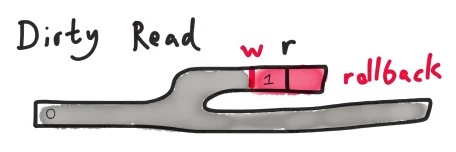
\includegraphics[width=0.7\linewidth]{img/dirty_read.png}
	\caption{Visualisierung eines Dirty Reads. Ist `w` eine Schreiboperation, die später zurückgerollt wird, dann ist `r` ein
		Dirty Read. \cite{jepsen_mongo_analysis}}
	\label{fig:dirty_read}
\end{figure}

Jepsen hat in MongoDB Version 2.6.7 einen Bug entdeckt, der im Fall gewisser Netzwerk-Unterbrechungen für eine kurze Zeit Dirty
Reads zulässt. Wenn der Leader-Knoten von der Mehrheit des Clusters getrennt wird, tritt dieser nach einem Timeout selbst zurück
und nimmt keine Schreiboperationen mehr entgegen. Wird allerdings vor diesem Timeout ein Wert über diesen Leader geschrieben, kann
dieser von dort auch gelesen werden, bevor er später zurückgerollt wird. Das liegt daran, dass in MongoDB damals neue
Schreiboperationen unter allen Konsistenzeinstellungen sofort vom Leader lesbar waren, noch bevor sie an eine Mehrheit des
Clusters repliziert wurden. \cite{jepsen_mongo_analysis}

Dieser Bug wird hier originalgetreu mittels der beschriebenen Raft Implementierung simuliert.

\subsubsection{B3: Election-Endlosschleife in MongoDB}
% ergebnis: funktioniert mit beiden bei 3 knoten (heuristic replay end unzuverlässig), bei mehr nur mit timing
Für die meisten Bugs bei Netzwerk-Unterbrechungen müssen Teile eines verteilten Systems vollständig voneinander getrennt sein. Es
gibt allerdings auch Bugs, die sich nur bei einer teilweisen Zertrennung eines Systems manifestieren. Ein Beispiel, welches
Alquraan et. al. \cite{analysis_of_network_partition_failures} nennen, ist ein Bug in MongoDB, welcher zu einer Schleife führt, in
der endlos neue Leader gewählt werden. MongoDB verwendet einen Verwaltungsknoten, um unentschiedene Elections zu entscheiden.
Tritt in einem Cluster mit zwei Replica-Knoten und einem Verwaltungsknoten eine Netzwerk-Unterbrechung wie in Abbildung
\ref{fig:partial_partition} auf, führt das dazu, dass Knoten A und B sich abwechselnd zum Leader wählen lassen, da sie jeweils nie
den Leader erreichen können, der Verwaltungsknoten aber immer an beiden Elections teilnehmen kann und den alten Leader dann über
den neuen Leader informiert. Dieser Bug manifestiert sich vollständig ohne Interaktionen durch einen Client von außen und
der Effekt verschwindet wieder, sobald die Netzwerk-Unterbrechung geheilt ist.

\begin{figure}[H]
	\centering
	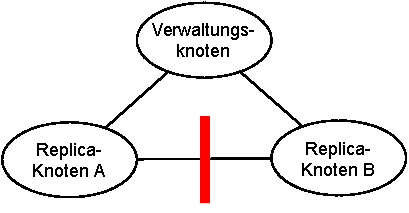
\includegraphics[width=0.6\linewidth]{img/ditm-Partitions.pdf}
	\caption{Visualisierung einer Netzwerk-Unterbrechung (rot), die in MongoDB eine Election-Endlosschleife auslösen konnte}
	\label{fig:partial_partition}
\end{figure}

Im Gegensatz zu MongoDB verwendet Raft keinen Verwaltungsknoten. Der beschriebene Bug kann dennoch realitätsnah in einem
Raft-Cluster nachgestellt werden, da in Raft jeder Knoten die Rolle einnehmen kann, die in MongoDB der Verwaltungsknoten für diesen
Bug spielt. Dazu müssen in Raft zwei Sicherheitsmechanismen ausgeschaltet werden:
\begin{itemize}
	\item dass Knoten nur für einen Leader gleichzeitig stimmen dürfen und
	\item dass Knoten nur Leader akzeptieren,  die in  wie sie selbst haben.
\end{itemize}

\subsubsection{B4: Split-Brain in Redis-Raft}
% ergebnis: funktioniert nur mit timing
Wenn ein Leader-basiertes System wie Raft mehr als einen Leader-Knoten gleichzeitig hat, wird dies als Split-Brain Situation
bezeichnet. Um diese Situationen zu vermeiden hat Raft verschiedene Sicherheitsmaßnahmen, wie dass jeder Knoten pro Term nur für
einen Leader stimmen darf. Die Maßnahme, dessen Fehlen diesen konkreten Bug ermöglicht, ist, dass das Entfernen eines Knotens aus
dem Cluster eine Mehrheitsentscheidung aller Knoten ist. Der Leader sollte also nicht in der Lage sein, einen Knoten zu entfernen,
ohne eine Bestätigung der Aktion von mindestens der Hälfte des Clusters zu erhalten.

Fehlt diese Einschränkung, ermöglicht das, eine Split-Brain Situation zu erzeugen, indem der Leader durch eine
Netzwerk-Unterbrechung vom Rest des Clusters getrennt wird und dann auf einmal angewiesen wird, alle anderen Knoten aus dem
Cluster zu entfernen. Das führt dazu, dass der alte Leader effektiv zu einen ein-Knoten Cluster wird, während die anderen Knoten
einen neuen Leader wählen und gemeinsam weiter als Cluster funktionieren. Das passiert, weil die anderen Knoten durch die
Netzwerk-Unterbrechung nie von ihrer Entfernung informiert werden und diese auch nicht bestätigen.

\subsubsection{B5: Unereichbare Daten}
% token login funktioniert in replays nicht, workaround: token lifetime wurde für Experimente auf 100 Tage gesetzt
% ergebnis: funktioniert mit beiden matchern
Das Startup-System verwendet ein eigenes, hierarchie-basiertes Authorisierungssystem. Dieses erlaubt es, Lese- und
Update-Operationen in jedem Service lokal zu authorisieren, für das Anlegen neuer Daten ist aber ein Request an den zentralen
Usermanagement-Service notwendig. Eine frühe Version dieses Authorisierungssystems hatte einen Bug, der dazu führte, dass neu
geschrieben Daten für Nutzer unzugänglich würden, sollte der Usermanagement-Service während der Schreiboperation unerreichbar
sein. Das lag daran, dass die Daten in diesem Fall einfach ohne die zur Authorisierung notwendige ID geschrieben wurden, die vom
Usermanagement-Service kommen sollte.

In neueren Versionen des Systems schlagen stattdessen Schreiboperationen in diesem Fall ganz fehl, um inkonsistente Datenstände zu
verhindern. Der Bug wurde hier in eine aktuelle Version des Systems wieder eingebaut, anstatt die alte Version des Systems zu
verwenden, da dies einfacher war, als kompatible alte Versionen aller Teile des Systems zu finden und zu konfigurieren.

\chapter{Ergebnisse}
Im Folgenden werden die Ergebnisse der einzelnen Experimente dargestellt und interpretiert. Im Anschluss folgt eine
zusammenfassende Diskussion der Evaluationsergebnisse.

\section{Request-Matching}
Die Ergebnisse der Experimente zur Evaluation den Request-Matchings sind gruppiert nach Art der Requests, so dass pro Tabelle
der Einfluss von Zufall in der Reihenfolge der Requests auf das Matching erkennbar wird. Die vom beschriebenen Bug im SUT
betroffenen Experimente sind in den Tabellen \ref{tab:get} und \ref{tab:get_ts} dargestellt und daran erkennbar, dass die Anzahl
der Requests von den vorgesehenen 10 und 100 abweicht. Interessant in diesen Experimenten ist zu beobachten, dass selbst bei
ungemischten Reqeust-Flüssen Fehler passieren, der Blick auf dem Median zeigt aber, dass dies nur in weniger als der Hälfte der
Durchführungen der Fall sein kann. Die Erklärung hierfür ist, dass durch den Bug ein vorangegangener Aufruf des SUT einen
Einfluss auf den nächsten haben kann, falls der letzte Request des vorangegangenen Aufrufs erfolgreich war und der erste Request
des neuen Aufrufs geblockt wird. In diesem Fall wird der erste Request erneut versucht, was in isolation selbst mit dem Bug
nicht passieren sollte. Tritt dieser Fall ein, verändert sich dadurch die Reihenfolge des gesamten Request-Flusses, da direkt am
Anfang ein zusätzlicher Request eingefügt wird, was zu den beobachteten Fehlern führt. Tabelle \ref{tab:get_nka} zeigt, dass
diese Fehler in der Tat durch den Bug ausgelöst werden, da sie nicht auftreten, wenn die Retries mittels no-keep-alive
verhindert werden. Des weiteren zeigt sich an den jeweils geringeren Request Anzahlen, dass der Bug deutlich weniger bei den
asynchronen Experimenten auftritt, vermutlich, weil dort weniger Verbindungen wiederverwendet werden, als im synchronen
Versuchsaufbau. Das seltenere Auftreten des Bugs erklärt auch die deutlich bessere Performance der heuristischen und Mix-Matcher
bei den asynchronen Experimenten im Vergleich zu den synchron gemischten in Tabelle \ref{tab:get}.
\begin{table}[H]
	\centering
	\caption{Ergebnisse der Request-Matching Experimente mit einfachen GET Requests}
	\label{tab:get}
	\begin{tabular}{|l|r|r|r|r|r|r|r|r|r|r|r|}
		\hline
		\multirow{2}{*}{Shuffle} & \multicolumn{2}{|c|}{num requests} & \multicolumn{2}{|c|}{heuristic} & \multicolumn{2}{|c|}{exact} & \multicolumn{2}{|c|}{mix} & \multicolumn{2}{|c|}{counting}                                    \\ \cline{2-11}
		                         & avg                                & med                             & avg                         & med                       & avg                            & med  & avg  & med  & avg  & med  \\ \hline
		no                       & 13.3                               & 13.5                            & 0.8                         & 0.0                       & 0.8                            & 0.0  & 0.8  & 0.0  & 1.7  & 0.0  \\ \hline
		no                       & 133.6                              & 133.0                           & 2.9                         & 0.0                       & 0.3                            & 0.0  & 2.9  & 0.0  & 15.2 & 0.0  \\ \hline
		1                        & 13                                 & 13.0                            & 1.7                         & 1.5                       & 2.2                            & 2.0  & 1.7  & 2.0  & 2.6  & 2.5  \\ \hline
		1                        & 133.2                              & 134.0                           & 22.7                        & 23.0                      & 39.1                           & 38.0 & 23.6 & 25.0 & 34.6 & 36.5 \\ \hline
		2                        & 13.5                               & 14.0                            & 2.5                         & 2.5                       & 3.0                            & 3.0  & 2.5  & 3.0  & 3.3  & 4.0  \\ \hline
		2                        & 131.5                              & 130.0                           & 22.5                        & 21.5                      & 40.3                           & 42.5 & 21.4 & 20.0 & 45.2 & 46.0 \\ \hline
		3                        & 13.3                               & 14.0                            & 2.0                         & 2.0                       & 3.5                            & 3.0  & 2.3  & 2.5  & 4.5  & 4.0  \\ \hline
		3                        & 135.1                              & 137.0                           & 25.8                        & 27.0                      & 42.2                           & 39.0 & 24.8 & 27.5 & 46.7 & 47.0 \\ \hline
		async                    & 13                                 & 14.0                            & 1.5                         & 1.5                       & 3.4                            & 4.0  & 1.4  & 1.0  & 5.5  & 5.0  \\ \hline
		async                    & 113.1                              & 111.5                           & 7.2                         & 6.5                       & 30.7                           & 31.0 & 7.0  & 6.0  & 68.2 & 67.0 \\ \hline
	\end{tabular}
\end{table}

Obwohl ein korrektes Request-Matching bei gemischter Reihenfolge durch den Bug effektiv unmöglich wird, da schlichtweg nicht die
gleichen Requests im Recording und im Replay sind, ist zu erkennen, dass der Heuristische und der Mix-Matcher sich hier insgesamt
deutlich besser verhalten, als die anderen beiden. Das ist in so fern relevant, dass auch in realen Szenarien durchaus
unterschiedliche Mengen an Requests in Recording und Replay sein können, beispielsweise wenn im Laufe eines Debugging Workflows
ein möglicher Bugfix getestet werden soll.

\begin{table}[H]
	\centering
	\caption{Ergebnisse der Request-Matching Experimente mit GET Requests mit Zeitstempeln}
	\label{tab:get_ts}
	\begin{tabular}{|l|r|r|r|r|r|r|r|r|r|r|r|}
		\hline
		\multirow{2}{*}{Shuffle} & \multicolumn{2}{|c|}{num requests} & \multicolumn{2}{|c|}{heuristic} & \multicolumn{2}{|c|}{exact} & \multicolumn{2}{|c|}{mix} & \multicolumn{2}{|c|}{counting}                                    \\ \cline{2-11}
		                         & avg                                & med                             & avg                         & med                       & avg                            & med  & avg  & med  & avg  & med  \\ \hline
		no                       & 13.6                               & 14.0                            & 0.7                         & 0.0                       & 0.9                            & 0.0  & 1.2  & 0.0  & 2.1  & 0.0  \\ \hline
		no                       & 134.7                              & 136.5                           & 19.6                        & 0.0                       & 19.0                           & 0.0  & 9.4  & 0.0  & 19.9 & 0.0  \\ \hline
		1                        & 13.8                               & 14.0                            & 3.3                         & 3.0                       & 3.0                            & 2.5  & 3.8  & 4.0  & 3.0  & 3.5  \\ \hline
		1                        & 135.4                              & 137.5                           & 37.0                        & 37.0                      & 36.2                           & 35.0 & 36.7 & 36.5 & 38.1 & 39.5 \\ \hline
		2                        & 13.4                               & 13.0                            & 3.7                         & 4.0                       & 4.3                            & 4.5  & 3.2  & 3.5  & 3.4  & 3.0  \\ \hline
		2                        & 134.1                              & 133.5                           & 42.0                        & 41.0                      & 43.1                           & 45.0 & 40.0 & 37.5 & 42.9 & 42.0 \\ \hline
		3                        & 13.2                               & 13.0                            & 4.1                         & 4.0                       & 5.3                            & 6.0  & 5.0  & 6.0  & 4.8  & 5.0  \\ \hline
		3                        & 134.5                              & 134.5                           & 48.8                        & 47.0                      & 48.3                           & 47.5 & 50.8 & 51.5 & 49.1 & 48.0 \\ \hline
		async                    & 13.7                               & 13.5                            & 5.0                         & 5.0                       & 5.6                            & 5.0  & 6.1  & 6.0  & 6.2  & 6.5  \\ \hline
		async                    & 113.4                              & 108.0                           & 60.9                        & 60.0                      & 65.2                           & 65.0 & 65.0 & 65.0 & 65.6 & 66.5 \\ \hline
	\end{tabular}
\end{table}

Tabelle \ref{tab:get_nka} zeigt, dass ditm problemlos mit stark gemischten Requests umgehen kann, sofern diese keine zufälligen
anderen komponenten enthalten. Auch hier verhalten sich wieder der Heutristische und der Mix-Matcher am besten, die beiden anderen
Matcher haben erneut deutliche Probleme.

\begin{table}[H]
	\centering
	\caption{Ergebnisse der Request-Matching Experimente mit GET Requests mit no-keep-alive header}
	\label{tab:get_nka}
	\begin{tabular}{|l|r|r|r|r|r|r|r|r|r|r|r|}
		\hline
		\multirow{2}{*}{Shuffle} & \multicolumn{2}{|c|}{num requests} & \multicolumn{2}{|c|}{heuristic} & \multicolumn{2}{|c|}{exact} & \multicolumn{2}{|c|}{mix} & \multicolumn{2}{|c|}{counting}                                  \\ \cline{2-11}
		                         & avg                                & med                             & avg                         & med                       & avg                            & med  & avg & med & avg  & med  \\ \hline
		no                       & 10                                 & 10.0                            & 0.0                         & 0.0                       & 0.0                            & 0.0  & 0.0 & 0.0 & 0.0  & 0.0  \\ \hline
		no                       & 100                                & 100.0                           & 0.0                         & 0.0                       & 0.0                            & 0.0  & 0.0 & 0.0 & 0.0  & 0.0  \\ \hline
		1                        & 10                                 & 10.0                            & 0.0                         & 0.0                       & 1.7                            & 2.0  & 0.0 & 0.0 & 4.2  & 3.5  \\ \hline
		1                        & 100                                & 100.0                           & 0.0                         & 0.0                       & 22.5                           & 22.5 & 0.0 & 0.0 & 40.2 & 41.0 \\ \hline
		2                        & 10                                 & 10.0                            & 0.0                         & 0.0                       & 2.5                            & 2.0  & 0.0 & 0.0 & 3.6  & 4.0  \\ \hline
		2                        & 100                                & 100.0                           & 0.0                         & 0.0                       & 25.4                           & 25.5 & 0.0 & 0.0 & 48.8 & 50.5 \\ \hline
		3                        & 10                                 & 10.0                            & 0.0                         & 0.0                       & 2.2                            & 2.0  & 0.0 & 0.0 & 5.0  & 5.0  \\ \hline
		3                        & 100                                & 100.0                           & 0.0                         & 0.0                       & 25.4                           & 25.0 & 0.0 & 0.0 & 52.2 & 53.0 \\ \hline
		async                    & 10                                 & 10.0                            & 0.0                         & 0.0                       & 2.5                            & 2.5  & 0.0 & 0.0 & 7.3  & 7.5  \\ \hline
		async                    & 100                                & 100.0                           & 0.0                         & 0.0                       & 22.4                           & 21.5 & 0.0 & 0.0 & 68.2 & 65.5 \\ \hline
	\end{tabular}
\end{table}

Treten in gemischten Request-Flüssen außerdem zufällige Komponenten auf, die das Request Matching zusätzlich erschweren, führt das
dazu, dass alle Requests-Matcher Fehler machen. Weiterhin sind der Heuristische und der Mix-Matcher mit Abstand am besten, einen
klaren Favoriten gibt es hier aber zwischen den beiden nicht, wie Tabelle \ref{tab:get_ts_nka} zeigt.

\begin{table}[H]
	\centering
	\caption{Ergebnisse der Request-Matching Experimente mit GET Requests mit Zeitstempeln und no-keep-alive header}
	\label{tab:get_ts_nka}
	\begin{tabular}{|l|r|r|r|r|r|r|r|r|r|r|r|}
		\hline
		\multirow{2}{*}{Shuffle} & \multicolumn{2}{|c|}{num requests} & \multicolumn{2}{|c|}{heuristic} & \multicolumn{2}{|c|}{exact} & \multicolumn{2}{|c|}{mix} & \multicolumn{2}{|c|}{counting}                                    \\ \cline{2-11}
		                         & avg                                & med                             & avg                         & med                       & avg                            & med  & avg  & med  & avg  & med  \\ \hline
		no                       & 10                                 & 10.0                            & 0.0                         & 0.0                       & 0.0                            & 0.0  & 0.0  & 0.0  & 0.0  & 0.0  \\ \hline
		no                       & 100                                & 100.0                           & 0.0                         & 0.0                       & 0.0                            & 0.0  & 0.0  & 0.0  & 0.0  & 0.0  \\ \hline
		1                        & 10                                 & 10.0                            & 3.4                         & 3.0                       & 4.3                            & 4.0  & 3.7  & 4.0  & 3.5  & 3.5  \\ \hline
		1                        & 100                                & 100.0                           & 40.7                        & 39.0                      & 43.8                           & 45.0 & 40.4 & 40.0 & 43.7 & 43.0 \\ \hline
		2                        & 10                                 & 10.0                            & 5.3                         & 5.5                       & 4.9                            & 5.0  & 5.0  & 4.5  & 4.4  & 4.0  \\ \hline
		2                        & 100                                & 100.0                           & 50.6                        & 51.5                      & 48.7                           & 48.0 & 50.9 & 52.5 & 48.4 & 48.0 \\ \hline
		3                        & 10                                 & 10.0                            & 4.6                         & 5.0                       & 4.3                            & 4.0  & 4.5  & 4.5  & 5.7  & 6.0  \\ \hline
		3                        & 100                                & 100.0                           & 48.5                        & 50.0                      & 50.8                           & 51.0 & 49.9 & 50.0 & 50.4 & 48.5 \\ \hline
		async                    & 10                                 & 10.0                            & 5.0                         & 5.0                       & 5.7                            & 6.0  & 4.9  & 4.5  & 7.7  & 7.5  \\ \hline
		async                    & 100                                & 100.0                           & 61.5                        & 60.5                      & 60.0                           & 61.0 & 62.4 & 62.5 & 68.7 & 69.0 \\ \hline
	\end{tabular}
\end{table}

Auch in den Experimenten in Tabelle \ref{tab:post}, die als zusätzliches Differenzierungsmerkmal drei unterschiedliche
Request-Body Längen über einen weiteren Parameter einführen, erziehlt kein Matcher selbst in den am leichtesten gemischten
Experimenten perfekte Ergebnisse. Trotzdem ist eine deutlich bessere Performance im Vergleich zu Tabelle \ref{tab:get_ts_nka} zu
erkennen. Vor allem in leicht gemischten Experimenten machen der Heuristische und der Mix-Matcher nur weniger als halb so viele
Fehler.

Insgesamt lässt sich sagen, dass die zwei komplexesten Matcher wie erwartet in allen Experimenten die besten Ergebnisse erzielen,
zwischen den beiden besteht dann aber kein relevanter Unterschied mehr, der in diesen Ergebnissen erkennbar wird.

\begin{table}[H]
	\centering
	\caption{Ergebnisse der Request-Matching Experimente mit POST Requests}
	\label{tab:post}
	\begin{tabular}{|l|r|r|r|r|r|r|r|r|r|r|r|}
		\hline
		\multirow{2}{*}{Shuffle} & \multicolumn{2}{|c|}{num requests} & \multicolumn{2}{|c|}{heuristic} & \multicolumn{2}{|c|}{exact} & \multicolumn{2}{|c|}{mix} & \multicolumn{2}{|c|}{counting}                                    \\ \cline{2-11}
		                         & avg                                & med                             & avg                         & med                       & avg                            & med  & avg  & med  & avg  & med  \\ \hline
		no                       & 10                                 & 10.0                            & 0.0                         & 0.0                       & 0.0                            & 0.0  & 0.0  & 0.0  & 0.0  & 0.0  \\ \hline
		no                       & 100                                & 100.0                           & 0.0                         & 0.0                       & 0.0                            & 0.0  & 0.0  & 0.0  & 0.0  & 0.0  \\ \hline
		1                        & 10                                 & 10.0                            & 0.7                         & 1.0                       & 3.1                            & 2.5  & 0.8  & 1.0  & 4.0  & 4.0  \\ \hline
		1                        & 100                                & 100.0                           & 8.0                         & 8.5                       & 42.0                           & 41.0 & 7.3  & 6.5  & 46.4 & 45.5 \\ \hline
		2                        & 10                                 & 10.0                            & 1.3                         & 1.0                       & 3.8                            & 3.5  & 1.5  & 1.0  & 3.9  & 4.0  \\ \hline
		2                        & 100                                & 100.0                           & 23.6                        & 22.5                      & 44.5                           & 44.5 & 24.9 & 25.0 & 46.6 & 46.5 \\ \hline
		3                        & 10                                 & 10.0                            & 2.3                         & 2.0                       & 4.4                            & 5.0  & 3.2  & 3.0  & 4.3  & 5.0  \\ \hline
		3                        & 100                                & 100.0                           & 31.2                        & 31.5                      & 46.6                           & 45.5 & 27.4 & 25.5 & 50.2 & 49.5 \\ \hline
		async                    & 10                                 & 10.0                            & 5.1                         & 5.0                       & 5.4                            & 6.0  & 4.4  & 4.5  & 7.0  & 7.0  \\ \hline
		async                    & 100                                & 100.0                           & 59.6                        & 59.0                      & 58.9                           & 60.0 & 58.6 & 58.5 & 66.7 & 67.5 \\ \hline
	\end{tabular}
\end{table}

Auch wenn die hier dargestellten Ergebnisse auf den ersten Blick zeigen, dass ditm sehr viele Fehler macht, sind diese Ergebnisse
doch positiv zu werten, wenn mit in Betracht gezogen wird, dass vorwiegend Szenarien verwendet wurden, die absichtlich schwierig
für ditm sein sollte, um die Limits der Request-Matcher herauszufinden. Die Erwartung ist, dass in den meisten realen Anwendungsfällen
nur sehr wenige gemischte Requests im gleichen Fluss auftreten, da ein Fluss immer genau den Verkehr zwischen nur zwei Knoten
abbildet. Reale Systeme senden vielmehr viele Requests zwischen unterschiedlichen Knoten des Systems, die ditm aufgrund
dessen von vornherein getrennt betrachtet und somit auch keine Fehler beim Matching macht. Die Experimente haben also gezeigt,
dass es durchaus Situationen geben kann, in denen ditm nicht funktioniert. Vor allem haben sie aber auch demonstriert, dass ditm
mit Schwierigkeiten umgehen kann, sofern diese nicht zu gehäuft auftreten. Leicht identifizierbare Reqeusts in stark gemischter
Reihenfolge sind kein Problem, genauso wie schwierig identifizierbare Reqests, die in größtenteils korrekter Reihenfolge
auftreten. Erst wenn beides zusammen kommt, funktioniert ditms Matching nicht mehr.

\section{Log-Matching}
Die Ergebnisse für das Log-Matching sind in Tabelle \ref{tab:logs} zusammengefasst.
Es ist anzumerken, dass die Anzahl der Fehler und auch der maximale Fehler bei den asynchronen Experimenten Schätzwerte sind, da durch
die asynchrone Natur der Experimente bei manchen Logs nicht eindeutig zu sagen ist, ob sie an richtiger Stelle stehen oder nicht.
Trotzdem zeigen die Werte demonstativ, dass das Log-Matching bei hoch asynchronen Prozessen mit vielen schnellen Logs
und Reqeusts an seine Grenzen kommen kann und dann effektiv unbrauchbar wird. Ganz im Gegenteil dazu stehen die Ergebnisse der
synchronen Experimente. Zwar gibt es auch hier durchaus Fehler, diese sind aber selten genug und vor allem klein genug, dass das Log-Matching
hier erheblich zur Effektivität von ditm als Debugging Werkzeug beitragen kann, wie sich auch schon im vorangegangenen Kapitel in
der Praxis gezeigt hat.
\begin{table}[H]
	\centering
	\caption{Ergebnisse der Log-Matching Experimente}
	\label{tab:logs}
	\begin{tabular}{|l|l|l|l|l|}
		\hline
		Anzahl Requests & Anzahl Logs & async & maximaler Fehler & Anzahl Fehler \\ \hline
		10              & 18          & nein  & 1                & 1             \\ \hline
		100             & 178         & nein  & 1                & 8             \\ \hline
		10              & 19          & ja    & 15               & 17            \\ \hline
		100             & 165         & ja    & 121              & 162           \\ \hline
	\end{tabular}
\end{table}

Eine weitere interessante Beobachtung ist, dass in dem längeren der beiden synchronen Experimenten die Fehler vorwiegend eng zusammen in Clustern
von zwei bis drei Fehlern direkt hintereinander auftreten. Bei den asynchronen Experimenten stehen sogar fast alle Logs ganz am Ende der Aufzeichnung
und fast alle Requests gemischt mit nur sehr wenigen Logs am Anfang. Beides deutet darauf hin, dass irgendwo in der Logging Pipeline möglicherweise
ein Buffer nicht schnell genug abgearbeitet wird und sich die Log-Nachrichten so anstauen können. Es ist außerdem naheliegend, dass nicht der ditm Proxy
selbst, welcher die Logs sammelt, den Flaschenhals bildet, sondern bereits der Docker Daemon oder noch wahrscheinlicher der verwendete HTTP-Log-Driver,
da die Zeitstempel, welche zur Sortierung der Tabelle von Reqeusts und Logs verwendet werden, in diesem Teil des Systems generiert werden.

\section{Debugging}
Alle der beschriebenen Bugs lassen sich mit Hilfe von ditm in Recordings und in Replays reproduzieren. Da insbesondere für die
Reproduktion der Bugs in Raft teilweise eine Reihe von Schritten notwendig ist, wurden hierfür Python Skripts geschrieben, die
ditm effektiv als Failure-Testing Tool verwenden und so ein Recording mit dem jeweiligen Bug erstellen. Tabelle \ref{tab:debug}
gibt einen Überblick darüber, welche Bugs anhand dieser Recordings mit welchem Matching-Mechanismus zuverlässig reproduzierbar
sind.

\begin{table}[H]
	\centering
	\caption{Überblick darüber, mit welchen Matchern welche Bugs zuverlässig in Replays reproduzierbar sind. *Nur in einem Cluster mit
		drei Knoten.}
	\label{tab:debug}
	\begin{tabular}{|l|l|l|}
		\hline
		Bug                                    & Heuristisch & Zeitlich \\ \hline
		B1: Doppelte Buchung                   & ja          & nein     \\ \hline
		B2: Dirty Reads in MongoDB             & nein        & ja       \\ \hline
		B3: Election Endlosschleife in MongoDB & ja*         & ja       \\ \hline
		B4: Split-Brain in Redis-Raft          & nein        & ja       \\ \hline
		B5: Unnerreichbare Daten               & ja          & ja       \\ \hline
	\end{tabular}
\end{table}

Die doppelte Buchung ist nur deshalb nicht mit den zeitbasierten Matcher reproduzierbar, weil der Prototyp ditm nicht die
notwendigen Optionen anbietet, um den Bug ohne zufallsgetriebene Netzwerk-Unterbrechungen zu erzeugen.

Ditm war mit dem ursprünglich konzipierten Request-Matching-Mechanismus nicht in der Lage, die Bugs, welche in Raft nachgestellt
wurden, deterministisch zu reproduzieren. Das liegt daran, dass Raft und ähnliche Systeme die grundlegende Annahme dieses Ansatzes
verletzen, dass das SUT unter gleichen Umständen auch die gleichen Nachrichten zwischen den gleichen Knoten versendet. Die
Ausnahme, dass Bug 3 in einem Cluster von drei Knoten mit dem heutristischen Matcher reproduzierbar ist, kommt allein daher, dass
es in der Konfiguration immer alle Knoten an dem Bug beteiligt sein müssen und somit immer die gleichen Nachrichten gesendet
werden.  Wird das gleiche Experiment in einem Cluster mit fünf Knoten durchgeführt, ist der Bug nur noch mit dem zeitbasierten
Matcher reproduzierbar.

Der zeitbasierte Matcher wurde als Reaktion auf die Ergebnisse dieser Versuche entwickelt. Der Nachteil dieses neuen
Mechanismus ist, dass dieser in der aktuellen Form nicht für Recordings funktioniert, die zufallsbasierte Netzwerk-Unterbrechungen
verwenden.

Eine wichtige Beobachtung bei Bug 5 ist, dass ditm grundsätzlich keine Token-basierte Authentifizierung während Replays unterstützt, da hierfür
Daten aus einer Response in den folgenden Requests mitgesendet werden müssen. Ditm hingegen sendet im Replay den exact gleichen
Request, wie im Recording und ignoriert einen neu generierten Token. Als Workaround wurde hier die Lebensdauer der Access-Token
des SUT auf mehrere Monate gesetzt, um ditm zu erlauben, diese während eines Replays wiederzuverwenden. Mit dieser Einstellung
hatte ditm keine Probleme, den Bug deterministisch zu reproduzieren.

\section{Erfahrungsbericht zu ditm als Debugger}
\label{chap:debugging_go}
% vielleicht code beispiel einfügen oder so
% mindestens absätze einfügen
Während der Entwicklung der Experimente zum Request-Matching trat ein relativ komplexer Bug in dem absichtlich einfach
gehaltenen SUT auf, welcher mit Hilfe von ditm identifiziert, untersucht und behoben werden konnte.

Schon bei einer ersten händischen Durchführung der ersten Experimente viel auf, dass etwas nicht stimmen konnte.
Nicht nur waren die Ergebnisse aus ditms Sicht unerwartet negativ, nach genauerem Hinsehen fanden sich in den Aufzeichnungen auch
teilweise deutlich mehr Requests, als für das jeweilige Experiment vorgesehen, was wiederum die schlechten Ergebnisse erklärte.
Die erste Intuition war, den Fehler in ditm zu suchen, immerhin handelte es sich um ein komplexes und wenig getestetes System.

Erst nachdem sich die Fehlersuche in ditm als früchtelos erwies, viel der Blick auf das augenscheinlich sehr einfache SUT.  Hier
erwies sich ditm tatsächlich als sehr geeignetes Debugging Werkzeug für das vorhandene Problem. Mit Hilfe der chronologischen
Darstellung von Requests und Logs konnte festgestellt werden, dass der verwendete HTTP Client unter sehr bestimmten Bedingungen
Retries für gescheiterte Requests sendet. Zu diesen Bedingungen zählt, dass der Request idempotent sein muss, POST Requests werden
also niemals wiederholt. Dass der Client Retries für idempotente Requests sendet, ist auch in der Dokumentation zu finden
\cite{go_transport_docs}. Das mit ditm beobachtete Verhalten ist damit allerdings noch nicht erklärt, da ein gescheiterter Request
nur dann wiederholt wird, wenn er
\begin{itemize}
    \item idempotent ist und
    \item auf einen erfolgreichen Request an das gleiche Ziel folgt.
\end{itemize}
Dieses Verhalten, dass Retries nur passieren, wenn die Verbindung bereits erfolgreich verwendet wurde,
ist nicht in der offiziellen Dokumentation dokumentiert \cite{go_transport_docs}, entspricht aber dem gewollten Verhalten, welches in
einer Commit-Nachricht in Googles Versionskontroll-System dokumentiert ist \cite{go_retry_commit}. Die mangelnde Dokumentation
wurde im Rahmen dieser Arbeit auf Golangs Issue-Tracker festgehalten und kann somit in Zukunft verbessert werden.

Für ditm ist dies insofern ein großer Erfolg, dass dieser Bug im SUT der erste zuvor unbekannte Bug ist, der mit ditm gefunden
wurde. Es handelt sich zwar nicht zusätzlich um einen neuen Bug in der Standartbibliothek von Go, aber trotzdem wurde auch hier
ein ähnlicher mentaler Schritt wie beim Debugging vollzogen. Es wurde mit Hilfe von ditm eine Diskrepanz zwischen dem erwarteten
und dem tatsächlichen Verhalten der Bibliothek gefunden und es konnten sogar die genauen Unterschiede im Verhalten korrekt
festgestellt werden.

\section{Diskussion}
% the interactive model is good at tightening the feedback loop

\chapter{Future Work}
% hier kommt future work, die ich als experte sehe, auch im kontext meiner arbeit

% keep and extend the idea of an interactive, graphical tool / debugger,
% while switching out failure mechanism for ssh, and extending to allow clock drift etc (like failify does it in docker)

% explore additional UI features: a builting graphical request 'builder',
% a smart diff tool for recordings / action sequences
% a drag and drop test case / replay editor to build predefined action sequences,
% enable using replays from an interactive session as an automated regression test

% vielleicht EBPF basiertes system, das wie proxy einzelne Requests blocken kann, aber auf jedem Knoten einzeln agiert?

\chapter{Fazit}

\printbibliography

\end{document}
